% \documentclass[answers]{exam}
% \usepackage{marvosym}

%...TikZ & PGF
\usepackage{pgfplots}
\pgfplotsset{compat=1.11}
\tikzset{>=latex}
\usetikzlibrary{calc,math}
\usepackage{tikzsymbols}
\usepgfplotslibrary{fillbetween}
\usetikzlibrary{decorations.markings} 
\usetikzlibrary{arrows.meta} %...APP2 for arrows as objects and images
\usetikzlibrary{backgrounds} %...For shading portions of graphs
\usetikzlibrary{patterns} %...Unit 5 Problems
\usetikzlibrary{shapes.geometric} %...For drawing cylinders in Unit 2
\tikzset{
    mark position/.style args={#1(#2)}{
        postaction={
            decorate,
            decoration={
                markings,
                mark=at position #1 with \coordinate (#2);
            }
        }
    }
} %...See https://tex.stackexchange.com/questions/43960/define-node-at-relative-coordinates-of-draw-plot

\tikzset{
    declare function = {trajectoryequation10(\x,\vi,\thetai)= tan(\thetai)*\x - 10*\x^2/(2*(\vi*cos(\thetai))^2);},
    declare function = {trajectoryequation(\x,\vi,\thetai)= tan(\thetai)*\x - 9.8*\x^2/(2*(\vi*cos(\thetai))^2);},
    declare function = {patheq(\x,\yi,\vi,\thetai)= \yi + tan(\thetai)*\x - 9.8*\x^2/(2*(\vi*cos(\thetai))^2);},
    declare function = {patheqten(\x,\yi,\vi,\thetai)= \yi + tan(\thetai)*\x - 10*\x^2/(2*(\vi*cos(\thetai))^2);} %like patheq but with gravity = 10
}

%...siunitx
\usepackage{siunitx}
\DeclareSIUnit{\nothing}{\relax}
\def\mymu{\SI{}{\micro\nothing} }
\DeclareSIUnit\mmHg{mmHg}
\DeclareSIUnit{\mile}{mi}
%...NOTE: "The product symbol between the number and unit is set using the quantity-product option."

%...Other
\usepackage{amsthm}
\usepackage{amsmath}
\usepackage{amssymb}
\usepackage{cancel}
\usepackage{subcaption}
\usepackage{dashrule}
\usepackage{enumitem}
\usepackage{fontawesome}
\usepackage{multicol}
\usepackage{glossaries}
%\numberwithin{equation}{section}
\numberwithin{figure}{section}
\usepackage{float}
\usepackage{twemojis} %...twitter emojis
\usepackage{utfsym}
\newcommand{\R}{\mathbb{R}} %...real number symbol
\usepackage{graphicx}
\graphicspath{ {../Figures/} }
\usepackage{hyperref}
\hypersetup{colorlinks=true,
    linkcolor=blue,
    filecolor=magenta,
    urlcolor=cyan,}
\urlstyle{same}
\newcommand{\hdashline}{{\hdashrule{\textwidth}{0.5pt}{0.8mm}}}
\newcommand{\hgraydashline}{{\color{lightgray} \hdashrule{0.99\textwidth}{1pt}{0.8mm}}}

%...Miscellaneous user-defined symbols
\newcommand{\fnet}{F_{\text{net}}} %...For net force
\newcommand{\bvec}[1]{\vec{\mathbf{#1}}} %...bold vector
\newcommand{\bhat}[1]{\,\hat{\mathbf{#1}}} %...bold hat vector
\newcommand{\que}{\mathord{?}}  %...Question mark symbol in equation env
%...Define thick horizontal rule for examples:
\newcommand{\hhrule}{\hrule\hrule}
\let\oldtexttt\texttt% Store \texttt
\renewcommand{\texttt}[2][black]{\textcolor{#1}{\ttfamily #2}}% 

%...For use in the exam document class
\newif\ifprintmetasolutions


%...Decreases space above and below align and gather enironment
\makeatletter
\g@addto@macro\normalsize{%
  \setlength\abovedisplayskip{-3pt}
  \setlength\belowdisplayskip{6pt} 
}
\makeatother





% \usepackage[margin=1in]{geometry}
\usepackage[figurewithin=none]{caption}
\usepackage{exam-randomizechoices}

\CorrectChoiceEmphasis{\color{red}\bfseries}
\renewcommand{\solutiontitle}{\noindent\textbf{\textcolor{red}{Solution:}}\enspace}

\usepackage{OutilsGeomTikz}
\usepackage{utfsym} %...Symbols in Unit 7 Problems
\usepackage{tabu} %...Symbols in Unit 7 Problems

%...For use in Unit 2            %    
\setlength{\columnsep}{2cm}      %
\setlength{\columnseprule}{1pt}  %
\usepackage[none]{hyphenat}      %
%%%%%%%%%%%%%%%%%%%%%%%%%%%%%%%%%

%...For use in Unit 11 on Waves:
\pgfdeclarehorizontalshading{visiblelight}{50bp}{  %
color(0.00000000000000bp)=(red);                   %
color(8.33333333333333bp)=(orange);                %
color(16.66666666666670bp)=(yellow);               %
color(25.00000000000000bp)=(green);                %
color(33.33333333333330bp)=(cyan);                 %
color(41.66666666666670bp)=(blue);                 %
color(50.00000000000000bp)=(violet)                %
}                                                  %

\newcommand{\checkbox}[1]{%
  \ifnum#1=1
    \makebox[0pt][l]{\raisebox{0.15ex}{\hspace{0.1em}\Large$\checkmark$}}%
  \fi
  $\square$%
}
%%%%%%%%%%%%%%%%%%%%%%%%%%%%%%%%%%%%%%%%%%%%%%%%%%%%

%...If using circuitikz package:
% \ctikzset{bipoles/battery1/height=0.5}
% \ctikzset{bipoles/battery1/width=0.25}
% \ctikzset{bipoles/resistor/height=0.15}
% \ctikzset{bipoles/resistor/width=0.4}
% \makenoidxglossaries

%...UNIT 1: CONSTANT MOTION

\newglossaryentry{scalar}{
    name=scalar,
    description={a quantity that has magnitude (and possibly sign) but no direction}
}

\newglossaryentry{magnitude}{
    name={magnitude},
    description={size or amount}
}

\newglossaryentry{vector}{
    name={vector},
    description={a quantity that has both magnitude and direction}
}

\newglossaryentry{tail}{
    name={tail},
    description={the starting point of a vector; the point opposite to the head or tip of the arrow}
}

\newglossaryentry{head}{
    name={head},
    description={the end point of a vector; the location of the vector's arrow; also referred to as the tip}
}

\newglossaryentry{head-to-tail method}{
    name={head-to-tail method},
    description={a method of adding vectors in which the tail of each vector is placed at the head of the previous vector}
}

\newglossaryentry{position}{
    name={position},
    description={the location of an object at any particular time}
}

\newglossaryentry{reference frame}{
    name={reference frame},
    description={a coordinate system from which the positions of objects are described}
}


\newglossaryentry{displacement}{
    name={displacement},
    description={the change in position of an object against a fixed axis}
}

\newglossaryentry{distance}{
    name={distance},
    description={the length of the path actually traveled between an initial and a final position}
}

\newglossaryentry{position vs. time graph}{
    name={position vs. time graph},
    description={a graph in which position is plotted on the vertical axis and time is plotted on the horizontal axis}
}

\newglossaryentry{speed}{
    name={speed},
    description={rate at which an object changes its location}
}

\newglossaryentry{average speed}{
    name={average speed},
    description={distance traveled divided by the time during which the motion occurs}
}

\newglossaryentry{velocity}{
    name={velocity},
    description={the speed and direction of an object}
}

\newglossaryentry{average velocity}{
    name={average velocity},
    description={displacement divided by the time during which the displacement occurs}
}

\newglossaryentry{velocity vs. time graph}{
    name={velocity vs. time graph},
    description={a graph in which velocity is plotted on the vertical axis and time is plotted on the horizontal axis}
}

\newglossaryentry{mass}{
    name=mass,
    description={the quantity of matter in a substance; the SI unit of mass is the kilogram}
}

\newglossaryentry{inertia}{
    name=inertia,
    description={the tendency of an object at rest to remain at rest, or for a moving object to remain in motion in a straight line and at a constant speed}
}

\newglossaryentry{Newton's first law of motion}{
    name={Newton's first law of motion},
    description={a body at rest remains at rest or, if in motion, remains in motion at a constant speed in a straight line, unless acted on by a net external force; also known as the law of inertia}
}

\newglossaryentry{momentum}{
    name={momentum},
    description={the product of a system's mass and velocity}
}

\newglossaryentry{momentum vs. time graph}{
    name={momentum vs. time graph},
    description={a graph in which momentum is plotted on the vertical axis and time is plotted on the horizontal axis}
}

\newglossaryentry{kinetic energy}{
    name={kinetic energy},
    description={energy of motion}
}

\newglossaryentry{joule}{
    name=joule,
    description={the metric unit for work and energy; equal to 1 newton meter ($\text{N}\cdot\text{m}$)}
}

\newglossaryentry{relative speed}{
    name={relative speed},
    description={how fast or slow an object appears to be moving to another object}
}

\newglossaryentry{relative velocity}{
    name={relative velocity},
    description={the rate at which an object changes position relative to another object}
}

%...UNIT 2: FORCE INTERACTIONS

\newglossaryentry{force}{
    name=force,
    description={a push or pull on an object with a specific magnitude and direction; can be represented by vectors; can be expressed as a multiple of a standard force; the SI unit of force is the Newton (N)}
}

\newglossaryentry{external force}{
    name=external force,
    description={a force acting on an object or system that originates outside of the object or system}
}

\newglossaryentry{free body diagram}{
    name=free body diagram,
    description={a diagram showing all external forces acting on a body}
}

\newglossaryentry{frictional force}{
    name=frictional force,
    description={an external force that acts opposite to the direction of motion or, for when there is no relative motion, in the direction needed to prevent slipping}
}

\newglossaryentry{applied force}{
    name={applied force},
    description={a contact force intentionally implied by a person on an object}
}


\newglossaryentry{gravitational force}{
    name=gravitational force, %...MY DEFINITION
    description={the downward force on an object due to the attraction by the Earth or other massive body}
}

\newglossaryentry{net force}{
    name=net force,
    description={the sum of all forces acting on an object or system}
}

\newglossaryentry{normal force}{
    name=normal force,
    description={that component of the contact force between two objects, which acts perpendicularly to and away from their plane of contact}
}

\newglossaryentry{tension}{
    name=tension,
    description={a pulling force that acts along a connecting medium, especially a stretched flexible connector, such as a rope or cable; when a rope supports the weight of an object, the force exerted on the object by the rope is called tension}
}

\newglossaryentry{spring force}{
    name=spring force, %...From district slides
    description={a force applied from a spring when it is either compressed or stretched}
}

%...UNIT 3: ACCELERATION

\newglossaryentry{acceleration}{
    name={acceleration},
    description={a change in velocity over time}
}

\newglossaryentry{average acceleration}{
    name={average acceleration},
    description={change in velocity divided by the time interval over which it changed}
}

%...UNIT 4:


\newglossaryentry{impulse}{
    name={impulse},
    description={average net external force multiplied by the time the force acts; equal to the change in momentum}
}

\newglossaryentry{impulse-momentum theorem}{
    name={impulse-momentum theorem},
    description={the impulse equals change in momentum}
}

\newglossaryentry{work}{
    name={work},
    description={force multiplied by distance}
}

%...UNIT 5: FORCE ANALYSIS

\newglossaryentry{Newton's universal law of gravitation}{
    name={Newton's universal law of gravitation},
    description={states that gravitational force between two objects is directly proportional to the product of their masses and inversely proportional to the square of the distance between them}
}

\newglossaryentry{gravitational constant}{
    name={gravitational constant},
    description={the proportionality constant in Newton's law of universal gravitation}
}

\newglossaryentry{weight}{
    name={weight},
    description={the force of gravity, $W$, acting on an object of mass $m$; defined mathematically as $W = mg$, where $g$ is the acceleration due to gravity}
}

\newglossaryentry{contact force}{
    name={contact force},
    description={a type of force that occurs when objects are physically in contact with each other}
}

%...UNIT 6: ONE-DIMENSIONAL MOTION

\newglossaryentry{free fall}{
    name=free fall,
    description={a situation in which the only force acting on an object is the force of gravity}
}

\newglossaryentry{kinematic equations}{
    name={kinematic equations},
    description={the 
    %five 
    equations that describe constant acceleration motion in terms of time, displacement, velocity, and acceleration}
}

%...UNIT 7: MOTION IN TWO DIMENSIONS

\newglossaryentry{projectile}{
    name={projectile},
    description={an object that travels through the air and experiences only acceleration due to gravity}
}

\newglossaryentry{projectile motion}{
    name={projectile motion},
    description={the motion of an object that is subject only to the acceleration of gravity}
}

\newglossaryentry{trajectory}{
    name={trajectory},
    description={the path of a projectile through the air}
}

\newglossaryentry{apex}{
    name={apex},
    description={the location on the trajectory at which the projectile reaches maximum height}
}

\newglossaryentry{hang time}{
    name={hang time},
    description={the amount of time that a projectile is in the air during projectile motion}
}

\newglossaryentry{horizontally launched projectile}{
    name={horizontally launched projectile},
    description={a projectile whose initial velocity is entirely in the horizontal direction}
}

\newglossaryentry{impact speed}{
    name={impact speed},
    description={the speed at which a projectile strikes the ground after being launched}
}

%...UNIT 8: CONSERVATION IN MECHANICAL SYSTEMS

\newglossaryentry{system}{
    name={system},
    description={one or more objects of interest for which only the forces acting on them from the outside are considered, but not the forces acting between them or inside them}
}

\newglossaryentry{energy}{
    name={energy},
    description={the ability to do work}
}

\newglossaryentry{potential energy}{
    name={potential energy},
    description={stored energy}
}

\newglossaryentry{gravitational potential energy}{
    name={gravitational potential energy},
    description={energy acquired by doing work against gravity}
}

\newglossaryentry{law of conservation of energy}{
    name={law of conservation of energy},
    description={states that energy is neither created nor destroyed}
}

\newglossaryentry{mechanical energy}{
    name={mechanical energy},
    description={kinetic plus potential energy}
}

\newglossaryentry{elastic collision}{
    name={elastic collision},
    description={a collision in which objects separate after impact and kinetic energy is conserved}
}

\newglossaryentry{inelastic collision}{
    name={inelastic collision},
    description={a collision in which kinetic energy is not conserved}
}

\newglossaryentry{isolated system}{
    name={isolated system},
    description={system in which the net external force is zero}
}

\newglossaryentry{law of conservation of momentum}{
    name={law of conservation of momentum},
    description={when the net external force is zero, the total momentum of the system is conserved or constant}
}

\newglossaryentry{perfectly inelastic collision}{
    name={perfectly inelastic collision},
    description={collision in which objects stick together after impact and kinetic energy is not conserved}
}

\newglossaryentry{recoil}{
    name={recoil},
    description={backward movement of an object caused by the transfer of momentum from another object in a collision}
}

%...UNIT 9: CONSERVATION OF CHARGE

\newglossaryentry{electric charge}{
    name={electric charge},
    description={a physical property of an object that causes it to be attracted toward or repelled from another charged object; each charged object generates and is influenced by a force called an electromagnetic force}
}

\newglossaryentry{electron}{
    name={electron},
    description={subatomic particle that carries one indivisible unit of negative electric charge}
}

\newglossaryentry{proton}{
    name={proton},
    description={subatomic particle that carries the same magnitude charge as the electron, but its charge is positive}
}

\newglossaryentry{electric field}{
    name={electric field},
    description={defines the force per unit charge at all locations in space around a charge distribution}
}

\newglossaryentry{law of conservation of charge}{
    name={law of conservation of charge},
    description={states that total charge is constant in any process}
}

\newglossaryentry{polarization}{
    name={polarization},
    description={separation of charge induced by nearby excess charge}
}

\newglossaryentry{Coulomb's law}{
    name={Coulomb's law},
    description={describes the electrostatic force between charged objects, which is proportional to the charge on each object and inversely proportional to the square of the distance between the objects}
}

\newglossaryentry{electric circuit}{
    name={electric circuit},
    description={physical network of paths through which electric current can flow}
}

\newglossaryentry{simple circuit}{
    name={simple circuit},
    description={a circuit with a single voltage source and a single resistor}
}

\newglossaryentry{electric current}{
    name={electric current},
    description={electric charge that is moving}
}


\newglossaryentry{Ohm's law}{
    name={Ohm's law},
    description={electric current is proportional to the voltage applied across a circuit or other path}
}

\newglossaryentry{resistance}{
    name={resistance},
    description={how much a circuit element opposes the passage of electric current; it appears as the constant of proportionality in Ohm’s law}
}

\newglossaryentry{resistor}{
    name={resistor},
    description={circuit element that provides a known resistance}
}

% \newglossaryentry{potential difference (or voltage)}{
%     name={potential difference (or voltage)},
%     description={change in potential energy of a charge moved from one point to another, divided by the charge; units of potential difference are joules per coulomb, known as volt}
% }

\newglossaryentry{voltage}{
    name={voltage},
    description={the electrical potential energy per unit charge; electric pressure created by a power source, such as a battery}
}

\newglossaryentry{electric power}{
    name={electric power},
    description={rate at which electric energy is transferred in a circuit}
}

\newglossaryentry{equivalent resistor}{
    name={equivalent resistor},
    description={resistance of a single resistor that is the same as the combined resistance of a group of resistors}
}

\newglossaryentry{in series}{
    name={in series},
    description={when elements in a circuit are connected one after the other in the same branch of the circuit}
}

\newglossaryentry{in parallel}{
    name={in parallel},
    description={when a group of resistors are connected side by side, with the top ends of the resistors connected together by a wire and the bottom ends connected together by a different wire}
}

\newglossaryentry{induction}{
    name={induction},
    description={creating an unbalanced charge distribution in an object by moving a charged object toward it (but without touching)}
}

%...UNIT 10: ELECTROMAGNETIC INDUCTION

\newglossaryentry{magnetic dipole}{
    name={magnetic dipole},
    description={term that describes magnets because they always have two poles: north and south}
}

\newglossaryentry{magnetic field}{
    name={magnetic field},
    description={directional lines around a magnetic material that indicates the direction and magnitude of the magnetic force}
}

\newglossaryentry{magnetic pole}{
    name={magnetic pole},
    description={part of a magnet that exerts the strongest force on other magnets or magnetic material}
}

\newglossaryentry{electromagnetic induction}{
    name={electromagnetic induction},
    description={rate at which energy is drawn from a source per unit current flowing through a circuit}
}


\newglossaryentry{Faraday's law}{
    name={Faraday's law},
    description={the means of calculating the emf in a coil due to changing magnetic flux}
}

\newglossaryentry{electromagnet}{
    name={electromagnet},
    description={device that uses electric current to make a magnetic field}
}

\newglossaryentry{transformer}{
    name={transformer},
    description={device that transforms voltages from one value to another}
}

\newglossaryentry{electric motor}{
    name={electric motor},
    description={device that transforms electrical energy into mechanical energy}
}

\newglossaryentry{generator}{
    name={generator},
    description={device that transforms mechanical energy into electrical energy}
}

%...UNIT 11: SIMPLE HARMONIC MOTION & WAVES

\newglossaryentry{wave}{
    name={wave},
    description={a disturbance that moves from its source and carries energy}
}

\newglossaryentry{wave velocity}{
    name={wave velocity},
    description={speed at which the disturbance moves; also called the propagation velocity or propagation speed}
}

\newglossaryentry{wavelength}{
    name={wavelength},
    description={distance between adjacent identical parts of a wave}
}

\newglossaryentry{wave cycle}{
    name={wave cycle},
    description={any portion of a wave encompassed by 1 wavelength}
}

\newglossaryentry{transverse wave}{
    name={transverse wave},
    description={a wave in which the disturbance is perpendicular to the direction of propagation}
}

\newglossaryentry{medium}{
    name={medium},
    description={the solid, liquid, or gas material through which a wave propagates}
}

\newglossaryentry{mechanical wave}{
    name={mechanical wave},
    description={wave that requires a medium through which it can travel}
}

\newglossaryentry{longitudinal wave}{
    name={longitudinal wave},
    description={wave in which the disturbance is parallel to the direction of propagation}
}

\newglossaryentry{constructive interference}{
    name={constructive interference},
    description={when two waves arrive at the same point exactly in phase; that is, the crests of the two waves are precisely aligned, as are the troughs}
}

\newglossaryentry{destructive interference}{
    name={destructive interference},
    description={when two identical waves arrive at the same point exactly out of phase that is precisely aligned crest to trough}
}

\newglossaryentry{oscillate}{
    name={oscillate},
    description={to move back and forth regularly between two points}
}

\newglossaryentry{amplitude}{
    name={amplitude},
    description={the maximum displacement from the equilibrium position of an object oscillating around the equilibrium position}
}

\newglossaryentry{frequency}{
    name={frequency},
    description={number of wave cycles per unit of time}
}

\newglossaryentry{simple harmonic motion}{
    name={simple harmonic motion},
    description={the oscillatory motion in a system where the net force can be described by Hooke’s law}
}

\newglossaryentry{simple harmonic oscillator}{
    name={simple harmonic oscillator},
    description={a device that oscillates in SHM,  such as a mass that is attached to a spring, where the restoring force is proportional to the displacement and acts in the direction opposite to the displacement}
}

\newglossaryentry{period}{
    name={period},
    description={the time it takes to complete one oscillation}
}

\newglossaryentry{electromagnetic wave}{
    name={electromagnetic wave},
    description={a radiant energy wave that consists of oscillating electric and magnetic fields}
}

\newglossaryentry{electromagnetic radiation}{
    name={electromagnetic radiation},
    description={radiant energy that consists of oscillating electric and magnetic fields}
}









%... Overview and Student Learning Expectations (OSLE)

\newglossaryentry{OSLE 6.1.a}{
    name={OSLE 6.1.a},
    description={compare the gravitational field strength on Earth to the acceleration due to gravity on Earth}
}

\newglossaryentry{OSLE 6.1.b}{
    name={OSLE 6.1.b},
    description={explain using universal gravitation and $F_\mathrm{net}=ma$ why all objects near Earth's surface fall at the same rate when in free fall}
}

\newglossaryentry{OSLE 6.1.c}{
    name={OSLE 6.1.c},
    description={explain the relationship between the mass, initial position, and initial velocity of an object in free fall on its final velocity and/or time in free fall}
}

\newglossaryentry{OSLE 6.1.d}{
    name={OSLE 6.1.d},
    description={describe the displacement, velocity, momentum, kinetic energy, and acceleration of an object in free fall that was dropped, thrown upward, or thrown downward using Multiple Representations}
}

\newglossaryentry{OSLE 6.1.e}{
    name={OSLE 6.1.e},
    description={relate the gravitational force, impulse, and work done on the object by the Earth to the object's change in velocity (acceleration), momentum, and kinetic energy}
}

        
\newglossaryentry{OSLE 6.2.a}{
    name={OSLE 6.2.a},
    description={describe what is known about an object's motion in a constant acceleration word problem using Multiple Representations}
}

\newglossaryentry{OSLE 6.2.b}{
    name={OSLE 6.2.b},
    description={solve for various unknown quantities utilizing kinematic equations when data is given in Multiple Representations for objects moving horizontally with constant acceleration}
}

\newglossaryentry{OSLE 6.3.c}{
    name={OSLE 6.3.c},
    description={solve for various unknown quantities utilizing kinematic equations when data is given in Multiple Representations for objects moving vertically with constant acceleration (free fall)}
}

\newglossaryentry{OSLE 6.4.d}{
    name={OSLE 6.4.d},
    description={solve multi-step problems that connect kinematic equations, the Law of Acceleration, Work-Energy Theorem, and/or the Impulse-Momentum Theorem}
}

\newglossaryentry{OSLE 7.1.a}{
    name={OSLE 7.1.a},
    description={compare the trajectory, hang time, max height, range, and final velocity of various projectiles that have different initial velocities, launch heights, launch angles, and masses, only varying one parameter at a time}
}

\newglossaryentry{OSLE 7.1.b}{
    name={OSLE 7.1.b},
    description={identify if and explain how the  initial velocity, launch height, launch angle, and mass of a projectile influence its motion---hang time, height, range, final velocity}
}

\newglossaryentry{OSLE 7.2.a}{
    name={OSLE 7.2.a},
    description={describe the vertical and horizontal motion of a projectile with a launch angle of zero using Multiple Representations}
}

\newglossaryentry{OSLE 7.2.b}{
    name={OSLE 7.2.b},
    description={illustrate the resultant motion of the projectile at any point in its trajectory as well as the relationship between the horizontal and vertical components using vector addition}
}

\newglossaryentry{OSLE 7.2.c}{
    name={OSLE 7.2.c},
    description={analyze and solve word problems about the motion of  horizontally launched projectiles using kinematic equations, vector addition, and  Multiple Representations}
}

\newglossaryentry{OSLE 7.3.a}{
    name={OSLE 7.3.a},
    description={describe the motion of an object moving with uniform circular motion in terms of centripetal force, centripetal acceleration, momentum, kinetic energy, and tangential velocity using Multiple Representations}
}

\newglossaryentry{OSLE 7.3.b}{
    name={OSLE 7.3.b},
    description={determine the centripetal force, mass, centripetal acceleration, tangential velocity, or radius of an object in circular motion}
}

\newglossaryentry{OSLE 7.4.a}{
    name={OSLE 7.4.a},
    description={predict the effects of changing the radius or mass of objects in orbiting systems using concepts of uniform circular motion and Newton’s law of universal gravitation}
}


\newglossaryentry{OSLE 8.1.a}{
    name={OSLE 8.1.a},
    description={identify multiple choices for a system given a scenario}
}

\newglossaryentry{OSLE 8.1.b}{
    name={OSLE 8.1.b},
    description={recognize that energy can be stored in the arrangement of particles or objects in a system as potential energy}
}

\newglossaryentry{OSLE 8.1.c}{
    name={OSLE 8.1.c},
    description={identify and calculate (i) gravitational potential energy and (ii) elastic potential energy when a system includes energy stored in the arrangement of its particles or objects}
}

\newglossaryentry{OSLE 8.1.d}{
    name={OSLE 8.1.d},
    description={compare the potential energy of a scenario for various choices of system}
}

\newglossaryentry{OSLE 8.1.e}{
    name={OSLE 8.1.e},
    description={identify, represent using multiple representations, and calculate the total mechanical energy present in a physical system}
}

\newglossaryentry{OSLE 8.1.f}{
    name={OSLE 8.1.f},
    description={predict the effects of changing the mass, velocity, height, gravitational field strength, spring constant, compression or stretching distance on the amount of $E_k$, $E_\mathrm{GP}$, and $E_\mathrm{SP}$}
}

\newglossaryentry{OSLE 8.1.g}{
    name={OSLE 8.1.g},
    description={calculate the total mechanical energy of a system}
}

\newglossaryentry{OSLE 8.2.a.i}{
    name={OSLE 8.2.a.i},
    description={identify, represent using multiple representations, and calculate the amount of energy (1) transformed from one storage mode to another within a system (including kinetic energy, potential energy, and thermal energy), (2) transferred from one object in the system to another in the system, and (3) entering/leaving a system due to work, heat, light, or sound}
}

\newglossaryentry{OSLE 8.2.b.i}{
    name={OSLE 8.2.b.i},
    description={explain the meaning of the Law of Conservation of Energy}
}

\newglossaryentry{OSLE 8.2.b.ii}{
    name={OSLE 8.2.b.ii},
    description={develop an energy formula for systems using energy bar charts and the Law of Conservation of Energy}
}

\newglossaryentry{OSLE 8.2.b.iii}{
    name={OSLE 8.2.b.iii},
    description=solve for various unknown quantities using the concept of the conservation of energy{}
}

\newglossaryentry{OSLE 8.2.c.i}{
    name={OSLE 8.2.c.i},
    description={know the definition of work as change in energy of a system}
}

\newglossaryentry{OSLE 8.2.c.ii}{
    name={OSLE 8.2.c.ii},
    description={know that power is work done divided by time}
}

\newglossaryentry{OSLE 8.3.a}{
    name={OSLE 8.3.a},
    description={calculate and compare the momentum, changes in momentum, force applied to and impulse on each object involved in a collision or explosion scenario}
}

\newglossaryentry{OSLE 8.3.b}{
    name={OSLE 8.3.b},
    description={represent using multiple representations, compare, and calculate the total momentum of a system before and after a collision or explosion scenario}
}

\newglossaryentry{OSLE 8.3.c}{
    name={OSLE 8.3.c},
    description={explain the meaning of the Law of Conservation of Momentum}
}

\newglossaryentry{OSLE 8.3.d}{
    name={OSLE 8.3.d},
    description={solve for unknown quantities using the concept of the conservation of momentum}
}


\newglossaryentry{OSLE 9.1.a}{
    name={OSLE 9.1.a},
    description={identify the particles that contribute positive, negative, or no charge in an atom}
}

\newglossaryentry{OSLE 9.1.b}{
    name={OSLE 9.1.b},
    description={recognize that neutral objects have even numbers of positive and negative charges}
}

\newglossaryentry{OSLE 9.1.c}{
    name={OSLE 9.1.c},
    description={determine the charge of an object given the number of protons and electrons}
}

\newglossaryentry{OSLE 9.1.d}{
    name={OSLE 9.1.d},
    description={predict if two objects will attract, repel, or have no interaction based on their charges}
}

\newglossaryentry{OSLE 9.1.e}{
    name={OSLE 9.1.e},
    description={draw the electric field surrounding single charges and pairs of charges}
}

\newglossaryentry{OSLE 9.2.a}{
    name={OSLE 9.2.a},
    description={recognize that charge is conserved: it cannot be created or destroyed, only transferred}
}

\newglossaryentry{OSLE 9.2.b}{
    name={OSLE 9.2.b},
    description={realize that only electrons are transferred during charging}
}

\newglossaryentry{OSLE 9.2.c}{
    name={OSLE 9.2.c},
    description={compare and contrast charging by induction and conduction}
}

\newglossaryentry{OSLE 9.2.d}{
    name={OSLE 9.2.d},
    description={explain how polarization temporarily charges a neutral object}
}

\newglossaryentry{OSLE 9.2.e}{
    name={OSLE 9.2.e},
    description={describe how an electroscope determines if objects are charged}
}

\newglossaryentry{OSLE 9.2.f}{
    name={OSLE 9.2.f},
    description={determine whether an object is negatively charged, positively charged, or neutral when given the charge of one object and a description or diagram representing how the charged object interacts with an object of unknown charge}
}

\newglossaryentry{OSLE 9.2.g}{
    name={OSLE 9.2.g},
    description={draw and describe the resulting distribution of charge for various scenarios of induction, conduction, and polarization}
}


\newglossaryentry{OSLE 9.3.a}{
    name={OSLE 9.3.a},
    description={draw the free body diagram for 2 charged objects showing the direction and relative magnitude of the electrical force acting on each object at various distances from each other}
}

\newglossaryentry{OSLE 9.3.b}{
    name={OSLE 9.3.b},
    description={describe how the electric force depends on the charges and the distance between them}
}

\newglossaryentry{OSLE 9.3.c}{
    name={OSLE 9.3.c},
    description={compare and contrast the electric force to the gravitational force}
}

\newglossaryentry{OSLE 9.3.d}{
    name={OSLE 9.3.d},
    description={predict how changing the charge or distance affects the electric force}
}


\newglossaryentry{OSLE 9.4.a}{
    name={OSLE 9.4.a},
    description={identify the necessary components for a simple circuit and discover different ways to light a bulb}
}

\newglossaryentry{OSLE 9.4.b}{
    name={OSLE 9.4.b},
    description={trace the conducting path through a simple circuit}
}

\newglossaryentry{OSLE 9.4.c}{
    name={OSLE 9.4.c},
    description={explain the concepts of current, resistance, voltage}
}

\newglossaryentry{OSLE 9.4.d}{
    name={OSLE 9.4.d},
    description={measure the current, resistance and voltage in a circuit using a multimeter, ammeter, current probe, etc}
}

\newglossaryentry{OSLE 9.4.e}{
    name={OSLE 9.4.e},
    description={calculate the voltage drop across, current through, or resistance of a circuit component using Ohm’s Law}
}

\newglossaryentry{OSLE 9.4.f}{
    name={OSLE 9.4.f},
    description={determine the change in current as the voltage or resistance is changed}
}

\newglossaryentry{OSLE 9.4.g}{
    name={OSLE 9.4.g},
    description={interpret electrical power as the rate at which electrical energy is being dissipated in the circuit}
}

\newglossaryentry{OSLE 9.4.h}{
    name={OSLE 9.4.h},
    description={relate the power rating/wattage of a light bulb to its brightness}
}


\newglossaryentry{OSLE 9.5.a}{
    name={OSLE 9.5.a},
    description={measure the current, resistance and voltage at various locations in a series circuit using a multimeter, ammeter, current probe, etc}
}

\newglossaryentry{OSLE 9.5.b}{
    name={OSLE 9.5.b},
    description={describe qualitatively and quantitatively the current flow throughout a series circuit}
}

\newglossaryentry{OSLE 9.5.c}{
    name={OSLE 9.5.c},
    description={calculate the equivalent resistance of multiple resistors in series}
}

\newglossaryentry{OSLE 9.5.d}{
    name={OSLE 9.5.d},
    description={calculate the equivalent voltage of batteries in series}
}

\newglossaryentry{OSLE 9.5.e}{
    name={OSLE 9.5.e},
    description={recognize that the sum of the voltage drops across resistors in series equals the total voltage of the power supply}
}

\newglossaryentry{OSLE 9.5.f}{
    name={OSLE 9.5.f},
    description={describe the energy transformations (transfers) occurring in a series circuit}
}

\newglossaryentry{OSLE 9.5.g}{
    name={OSLE 9.5.g},
    description={determine (i) current through, voltage drop across, and power of each component, and (i) total current of circuit, when given a series circuit diagram}
}


\newglossaryentry{OSLE 9.6.a}{
    name={OSLE 9.6.a},
    description={measure the current, resistance and voltage at various locations in a parallel circuit using a multimeter, ammeter, current probe, etc}
}

\newglossaryentry{OSLE 9.6.b}{
    name={OSLE 9.6.b},
    description={recognize that the current going into a junction is equal to the current coming out of it}
}

\newglossaryentry{OSLE 9.6.c}{
    name={OSLE 9.6.c},
    description={describe qualitatively and quantitatively the current flow throughout a parallel circuit}
}

\newglossaryentry{OSLE 9.6.d}{
    name={OSLE 9.6.d},
    description={recognize that the voltage drops across each resistor are equal to the voltage of the power supply}
}

\newglossaryentry{OSLE 9.6.e}{
    name={OSLE 9.6.e},
    description={describe advantages and disadvantages of parallel circuits compared to series circuits}
}

\newglossaryentry{OSLE 9.6.f}{
    name={OSLE 9.6.f},
    description={calculate the equivalent resistance of multiple resistors in parallel}
}

\newglossaryentry{OSLE 9.6.g}{
    name={OSLE 9.6.g},
    description={calculate the equivalent voltage of batteries in parallel}
}

\newglossaryentry{OSLE 9.6.h}{
    name={OSLE 9.6.h},
    description={describe the energy transformations (transfers) occurring in a parallel circuit}
}

\newglossaryentry{OSLE 9.6.i}{
    name={OSLE 9.6.i},
    description={determine the (i) current through, voltage drop across, and power of each component, and (ii) total current of circuit, when given a series circuit diagram}
}


\newglossaryentry{OSLE 9.7.a}{
    name={OSLE 9.7.a},
    description={determine whether elements of a combination circuit have the same current or voltage}
}

\newglossaryentry{OSLE 9.7.b}{
    name={OSLE 9.7.b},
    description={predict which bulbs will light if switches are open or closed}
}








% \setrandomizerseed{1}

% \firstpageheader{Physics}{Unit 2: Force Interactions}{Problems}
% \runningheader{}{}{}


\documentclass[../main-physics-problems.tex]{subfiles}

\begin{document}

\subsection{Interacting Objects}

\subsubsection{Types of Force}
\subsubsection{Representing Force Pairs in Interactions}
\subsubsection{Force Pairs as Two Forces of the Same Type}
\subsubsection{Instances in which Forces are Not a Force Pair}

\subsection{Constant Motion Model Based on Forces}

\subsubsection{Free-Body Diagrams}
\subsubsection{Effects of Balanced and Unbalanced Forces}
\subsubsection{Constant and Changing Velocity, Momentum, Kinetic Energy, and Forces}

\begin{questions}

\question
What is a force?

% \begin{solution}
%     A \gls{force} is \glsdesc{force}.
% \end{solution}

\question
What are some examples of a force?

\begin{solution}
    Answers may vary.

    \begin{itemize}[itemsep=0pt]
        \item Earth pulling down on a falling apple. 
        \item A chair pushing up on a person.
        \item A magnet attracting another magnet.
        \item Friction acting on a sliding person.
    \end{itemize}
\end{solution}

\question
What are some types of forces?

\begin{solution}
    Answers may vary.

    \begin{itemize}[itemsep=0pt]
        \item contact (applied) force
        \item magnetic force
        \item gravitational force
        \item tension force
        \item friction force
        \item normal force
    \end{itemize}
\end{solution}

\question
Can an object put a force on itself? %...Kind of a vague question. If you press your hand against your chest, you are putting a force on yourself.

\begin{solution}
    No. Force interactions occur between two objects.
\end{solution}

\question
\begin{parts}
\part What is the base SI unit of force? (What is the unit of measurement?)

\begin{solution}
    The newton (N).
\end{solution}

\part Express this unit in terms of the fundamental units (kg, m, s).

\begin{solution}
    One newton is equal to a kilogram multiplied by a meter per second squared:

    \begin{equation*}
        \SI{1}{N} = 1 \frac{\mathrm{kg}\cdot \mathrm{m}}{\mathrm{s}^2}
    \end{equation*}
\end{solution}
\end{parts}


\question
Two teams play tug-of-war. Team Red pushes right on a cart with a force of \SI{70}{newtons}. Team Blue applies a \SI{50}{N} leftward force. Draw a sketch of the forces and calculate the net force on the cart.

\begin{solution}
\begin{center}    

\begin{tikzpicture}
    \fill (0,0) circle (3pt);
    \begin{scope}[x=2]
        \draw[thick,->,left=5] (0,0) -- (-50,0) node[left] {\SI{50}{N}};
        \draw[thick,->,right=5] (0,0) -- (70,0) node[right] {\SI{70}{N}};
    \end{scope}
\end{tikzpicture}

\begin{equation*}
    F_{\text{net}} = 70 - 50 = \SI{20}{N} 
\end{equation*}
\end{center}
\end{solution}


\question
Spongebob and Patrick each apply a 50-newton rightward force on a treasure chest. Mr.~Krabs applies a \SI{75}{N} leftward force. 

\begin{parts}
\part Draw a sketch of the forces on the chest.

\begin{solution}
\begin{center}
    \begin{tikzpicture}
    \fill (0,0) circle (3pt);
        \begin{scope}[x=2,y=2]
            \draw[thick,->,left=5] (0,0) -- (-75,0) node[above,pos=0.5] {\SI{75}{N}};
            \draw[thick,->,above=3,right=4] (0,0) -- (50,0) node[above,pos=0.5] {\SI{50}{N}};
            \draw[thick,->,below=3,right=4] (0,0) -- (50,0) node[below,pos=0.5] {\SI{50}{N}};
        \end{scope}
    \end{tikzpicture}
\end{center}
\end{solution}

\part Calculate the net force on it.

\begin{solution}
\begin{equation*}
    F_{\text{net}} = 50 + 50 - 75 = \SI{25}{N}
\end{equation*}
\end{solution}
\end{parts}


\question 
Three forces act on an object. What is the magnitude and direction of the net force?

\begin{figure}[H]
    \centering
    \begin{tikzpicture}
    \fill (0,0) circle (3pt);
        \begin{scope}[x=2,y=2]
            \draw[thick,->,above=3,left=4] (0,0) -- ++(-63,0) node[above,pos=0.5] {\SI{63}{N}};
            \draw[thick,->,below=3,left=4] (0,0) -- ++(-73,0) node[below,pos=0.5] {\SI{73}{N}};
            \draw[thick,->,right=4] (0,0) -- ++(98,0) node[above,pos=0.5] {\SI{98}{N}};
        \end{scope}
    \end{tikzpicture}
\end{figure}

\begin{solution}
    \begin{equation*}
        F_{\text{net}} = 98 - 63 -73 = \SI{-38}{N}
    \end{equation*}
\end{solution}

\question
Four forces act on an object. Find the magnitude and direction of the net force.

\begin{center}
    \begin{tikzpicture}
        \fill (0,0) circle (3pt);
        \begin{scope}[x=2,y=2]
            \draw[thick,above=3,->,right=3] (0,0) -- (49,0) node[above,pos=0.5] {49\,N};
            \draw[thick,below=3,->,right=3] (0,0) -- (67,0) node[below,pos=0.5] {67\,N};
            \draw[thick,above=3,->,left=3] (0,0) -- (-22,0) node[above,pos=0.5] {22\,N};
            \draw[thick,below=3,->,left=3] (0,0) -- (-36,0) node[below,pos=0.5] {36\,N};
        \end{scope}
    \end{tikzpicture}
\end{center}


\begin{solution}
    \begin{equation*}
        F_{\text{net}} = 49 + 67 - 22 - 36 = \SI{58}{N}
    \end{equation*}
\end{solution}

\question
The net force on an object is $\bvec{F}_{\text{net}} = \SI{-25}{N}$. If the applied force is \SI{-46}{N}, what is the magnitude of the frictional force $f$? 

\begin{center}
    \begin{tikzpicture}
        \fill (0,0) circle (3pt);
        \begin{scope}[x=2,y=2]
            \draw[thick,->,left=5] (0,0) -- (-46,0) node[left] {$F_a$}; 
            \draw[thick,->,right=5] (0,0) -- (21,0) node[right] {$f$};
        \end{scope}
    \end{tikzpicture}
\end{center}

\begin{solution}
    \begin{align*}
        \bvec{F}_{\text{net}} &= f - F_a \\[1ex]
        -25 &= f - 46\\[1ex]
        - 25 + 46 &= f\\[1ex]
        f &= \SI{21}{N}
    \end{align*}
\end{solution}

\clearpage
\begin{EnvUplevel}
    \subsection{Force Pairs}
\end{EnvUplevel}

\question
A small car is at rest at a stoplight. A large truck rear-ends the small car. Why is the force experienced by the car greater than the force experienced by the truck?

\begin{randomizechoices}
    \choice The car has less mass; the less massive object experiences the greater force.
    \choice The car is at rest; the object with the smallest speed experiences the greater force.
    \choice Nonsense! The truck actually experiences a greater force than the car.
    \correctchoice Nonsense! Both the car and the truck experience the same amount of force.    
\end{randomizechoices}

\question
During a football game, a large lineman delivers a vicious hit to the opposing team’s quarterback. Why is the force experienced by the quarterback greater than the force experienced by the lineman?

\begin{randomizechoices}
    \choice The quarterback has less mass; the less massive object experiences the greater force.
    \choice The quarterback is stationary; an object at rest always experiences the greater force.
    \choice Nonsense! The lineman actually experiences a greater force than the quarterback.
    \correctchoice Nonsense! The lineman and the quarterback experience the same amount of force.    
\end{randomizechoices}

\question
A physics student sits in a chair. The chair pushes up on the student's body. Identify the other force of the interaction force pair.

\begin{randomizechoices}
    \choice The student's body pushes down on the Earth.
    \choice The Earth pulls down on the student's body.
    \choice The student's body pulling up on the Earth.
    \correctchoice The student's body pushing down on the chair.    
\end{randomizechoices}

\question
After missing a layup, Jonny expresses his anger by hitting the wall.  The reaction force to the force of Jonny's palm hitting the wall is\dots 

\begin{randomizechoices}
    \choice Jonny's palm stops
    \choice the wall forcing itself
    \choice Jonny's palm forcing itself
    \correctchoice the wall forcing Johnny's palm
    \choice the loud sound that is produced
\end{randomizechoices}

\question
A quiet moment during a test is interrupted as a physics book falls from a table and strikes the floor.  The reaction force to the force of the Earth pulling the book downwards is\dots 

\begin{randomizechoices}
    \choice the book hits the floor
    \choice the force of gravity on the book
    \choice the floor pushes up on the book
    \choice the sound of the impact with the floor
    \correctchoice the book exerts an upward pull on the Earth
\end{randomizechoices}

\clearpage
\begin{EnvUplevel}
    \subsection{Interactions of Objects}
\end{EnvUplevel}

\question
Consider a book at rest on a table.


\begin{center}

\begin{tikzpicture}
    \draw[fill=black!20] (0,0) rectangle ++(4,0.4);
    \draw[fill=black!20] (0.5,0) rectangle ++(0.2,-2);
    \draw[fill=black!20] (3.3,0) rectangle ++(0.2,-2);
    \node[above=2.9mm] at (2,0) {\twemoji[height=1cm]{blue book}};
\end{tikzpicture}
\hspace{1cm}
\begin{tikzpicture}
    \coordinate (earth) at (0,0); 
    \coordinate (table) at ({4},0); 
    \coordinate (book) at ({4*cos(60)},{4*sin(60)}); 
    \draw (book) node[above] {book};
    \draw (table) node[right] {table};
    \draw (earth) node[left] {earth};
    \draw[ultra thick,<->] (book)  -- (table) node[right=3pt,pos=0.1] {$F_\text{book-table}$} node[right=3pt,pos=0.8] {$F_\text{table-book}$};
    \draw[ultra thick,<->] (book) -- (earth) node[left=3pt,pos=0.1] {$F_\text{book-earth}$} node[left=3pt,pos=0.8] {$F_\text{earth-book}$};
    \draw[ultra thick,<->] (earth) -- (table) node[below=3pt,pos=0.2] {$F_\text{earth-table}$} node[below=3pt] {$F_\text{table-earth}$};
\end{tikzpicture}
\end{center}

\begin{parts}
    \part What are the force pairs in this scenario?
    
\begin{solution}
    There are three pairs.

    \begin{enumerate}
        \item The force on the book by the table ($F_\text{book-table}$) and the force on the table by the book ($F_\text{table-book}$)
        \item $F_\text{book-earth}$ and $F_\text{earth-book}$
        \item $F_\text{table-earth}$ and $F_\text{earth-table}$
    \end{enumerate}
\end{solution}

\part What are the force types?

\begin{solution}
    $F_\text{book-table}$ is the normal force, and $F_\text{table-book}$ is the reaction pair of the normal force.

    $F_\text{book-earth}$ and $F_\text{earth-book}$ are gravitational forces due to the mutual attraction of earth and book. Likewise, $F_\text{table-earth}$ and $F_\text{earth-table}$ are gravitational forces.
\end{solution}

\end{parts}

\question
What are the three force pairs and types involved in a person tugging a rope?

\begin{center}
    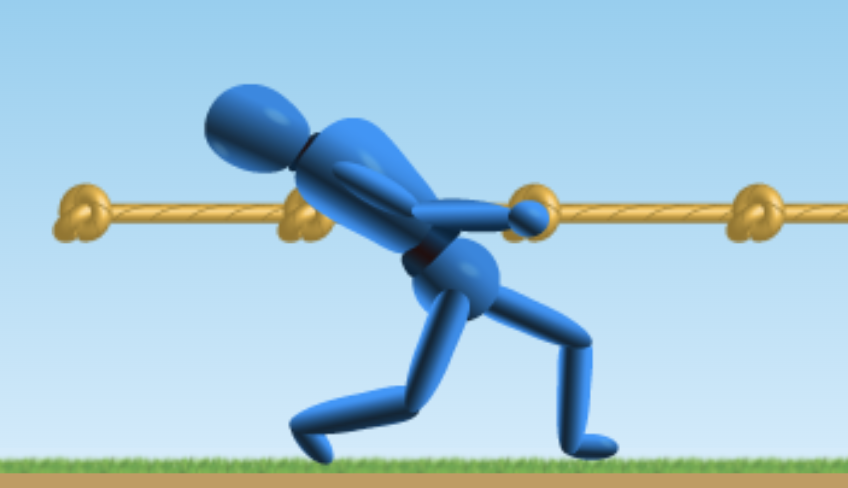
\includegraphics[width=5cm]{documents/figures/2.3-person-rope.png}
    \hspace{1cm}
    \begin{tikzpicture}
        \coordinate (earth) at (0,0); 
        \coordinate (rope) at ({4},0); 
        \coordinate (person) at ({4*cos(60)},{4*sin(60)}); 
        \draw (person) node[above] {person};
        \draw (rope) node[right] {rope};
        \draw (earth) node[left] {earth};
        \draw[ultra thick,<->] (person)  -- (rope);% node[right=3pt,pos=0.1] {$F_\text{person-rope}$} node[right=3pt,pos=0.8] {$F_\text{rope-person}$};
        \draw[ultra thick,<->] (person) -- (earth);% node[left=3pt,pos=0.1] {$F_\text{person-earth}$} node[left=3pt,pos=0.8] {$F_\text{earth-person}$};
        \draw[ultra thick,<->] (earth) -- (rope);% node[below=3pt,pos=0.2] {$F_\text{earth-rope}$} node[below=3pt] {$F_\text{rope-earth}$};
    \end{tikzpicture}
\end{center}

\begin{solution}
    \begin{center}
        \begin{tikzpicture}
            \coordinate (earth) at (0,0); 
            \coordinate (rope) at ({4},0); 
            \coordinate (person) at ({4*cos(60)},{4*sin(60)}); 
            \draw (person) node[above] {person};
            \draw (rope) node[right] {rope};
            \draw (earth) node[left] {earth};
            \draw[ultra thick,<->] (person)  -- (rope) node[right=3pt,pos=0.1] {$F_\text{person-rope}$} node[right=3pt,pos=0.8] {$F_\text{rope-person}$};
            \draw[ultra thick,<->] (person) -- (earth) node[left=3pt,pos=0.1] {$F_\text{person-earth}$} node[left=3pt,pos=0.8] {$F_\text{earth-person}$};
            \draw[ultra thick,<->] (earth) -- (rope) node[below=3pt,pos=0.2] {$F_\text{earth-rope}$} node[below=3pt] {$F_\text{rope-earth}$};
        \end{tikzpicture}
    \end{center}

$F_\text{person-earth}$ and $F_\text{earth-person}$ involve gravity and friction.

$F_\text{person-rope}$ and $F_\text{rope-person}$ involve tension and friction.

$F_\text{earth-rope}$ and $F_\text{rope-earth}$ involve gravity.


\end{solution}

\question
An air hockey puck glides across an air hockey table at a constant velocity.

% \begin{center}
%     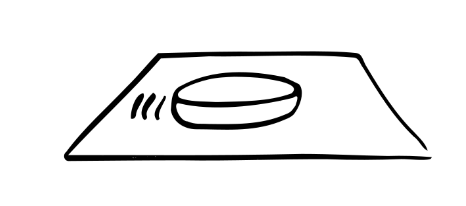
\includegraphics[width=4cm]{documents/figures/2.3-hockey.png}
% \end{center}

\begin{center}
\begin{tikzpicture}
\node[cylinder, 
    draw = black, 
    % text = purple,
    cylinder uses custom fill, 
    cylinder body fill = lightgray, 
    cylinder end fill = gray,
    minimum width = 3cm,
    minimum height = 1cm,
    aspect = 1.5, 
    shape border rotate = 90] (c) at (0,0) {};
\end{tikzpicture}
\end{center}

\begin{parts}
\part List all forces. Label each as a field or contact force.

\begin{solution}
    \begin{enumerate}
        \item The force on the puck by the table ($F_\text{puck-table}$) and the force on the table by the puck ($F_\text{table-puck}$). These are contact forces.
        \item $F_\text{puck-earth}$ and $F_\text{earth-puck}$. These are gravitational (field) forces.
        \item $F_\text{table-earth}$ and $F_\text{earth-table}$. These are gravitational (field) forces.
    \end{enumerate}
\end{solution}

\part Between what two objects does each force interact?

\begin{solution}
    \begin{enumerate}
        \item $F_\text{puck-table}$ and $F_\text{table-puck}$ interact between the puck and table.
        \item $F_\text{puck-earth}$ and $F_\text{earth-puck}$ interact between the puck and earth.
        \item $F_\text{table-earth}$ and $F_\text{earth-table}$ interact between the table and earth.
    \end{enumerate}
\end{solution}

\part Draw the force pairs and force schema.

\begin{solution}
\phantom{.}

\begin{center}
\begin{tikzpicture}
    \coordinate (earth) at (0,0); 
    \coordinate (table) at ({4},0); 
    \coordinate (puck) at ({4*cos(60)},{4*sin(60)}); 
    \draw (puck) node[above] {puck};
    \draw (table) node[right] {table};
    \draw (earth) node[left] {earth};
    \draw[ultra thick,<->] (puck)  -- (table) node[right=3pt,pos=0.1] {$F_\text{puck-table}$} node[right=3pt,pos=0.8] {$F_\text{table-puck}$};
    \draw[ultra thick,<->] (puck) -- (earth) node[left=3pt,pos=0.1] {$F_\text{puck-earth}$} node[left=3pt,pos=0.8] {$F_\text{earth-puck}$};
    \draw[ultra thick,<->] (earth) -- (table) node[below=3pt,pos=0.2] {$F_\text{earth-table}$} node[below=3pt] {$F_\text{table-earth}$};
\end{tikzpicture}    
\end{center}

\end{solution}
\end{parts}

\clearpage
\question
A woman is doing a handstand.

\begin{center}
    
\includegraphics[width=4cm]{documents/figures/2.3-woman.png}
\end{center}

\begin{parts}
    \part List all forces. Label each as a field or contact force.

\begin{solution}
    \begin{enumerate}
        \item The force on the woman by the floor ($F_\text{woman-floor}$) and the force on the floor by the woman ($F_\text{floor-woman}$). These are contact forces.
        \item $F_\text{woman-earth}$ and $F_\text{earth-woman}$. These are gravitational (field) forces.
    \end{enumerate}
\end{solution}

\part Between what two objects does each force interact?

\begin{solution}
    \begin{enumerate}
        \item $F_\text{woman-floor}$ and $F_\text{floor-woman}$ interact between the woman and floor.
        \item $F_\text{woman-earth}$ and $F_\text{earth-woman}$ interact between the woman and earth.
        \item $F_\text{floor-earth}$ and $F_\text{earth-floor}$ interact between the floor and earth.
    \end{enumerate}
\end{solution}


\part Draw the force pairs and the force schema.
\begin{solution}
\phantom{.}

\begin{center}
\begin{tikzpicture}
    \coordinate (earth) at (0,0); 
    \coordinate (floor) at ({4},0); 
    \coordinate (woman) at ({4*cos(60)},{4*sin(60)}); 
    \draw (woman) node[above] {woman};
    \draw (floor) node[right] {floor};
    \draw (earth) node[left] {earth};
    \draw[ultra thick,<->] (woman)  -- (floor) node[right=3pt,pos=0.1] {$F_\text{woman-floor}$} node[right=3pt,pos=0.8] {$F_\text{floor-woman}$};
    \draw[ultra thick,<->] (woman) -- (earth) node[left=3pt,pos=0.1] {$F_\text{woman-earth}$} node[left=3pt,pos=0.8] {$F_\text{earth-woman}$};
    \draw[ultra thick,<->] (earth) -- (floor) node[below=3pt,pos=0.2] {$F_\text{earth-floor}$} node[below=3pt] {$F_\text{floor-earth}$};
\end{tikzpicture}
\end{center}


\end{solution}

\end{parts}

\question
A climber is supported by a rope.

\begin{center}
    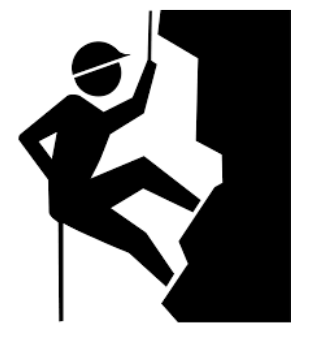
\includegraphics[width=4cm]{documents/figures/2.3-climber.png}
\end{center}

\begin{parts}
\part List all forces. Label each as a field or contact force.

\begin{solution}
    \begin{enumerate}
        \item The force on the climber by the rope ($F_\text{climber-rope}$) and the force on the rope by the climber ($F_\text{table-puck}$). These are contact forces, specifically tension and friction.
        \item $F_\text{climber-earth}$ and $F_\text{earth-climber}$. These are gravitational (field) forces.
        \item $F_\text{rope-earth}$ and $F_\text{earth-rope}$. These are gravitational (field) forces.
    \end{enumerate}
\end{solution}

\part Between what two objects does each force interact?

\begin{solution}
    \begin{enumerate}
        \item $F_\text{climber-rope}$ and $F_\text{rope-climber}$ interact between the climber and rope.
        \item $F_\text{climber-earth}$ and $F_\text{earth-climber}$ interact between the climber and earth.
        \item $F_\text{rope-earth}$ and $F_\text{earth-rope}$ interact between the rope and earth.
    \end{enumerate}
\end{solution}

\part Draw the force pairs and the force schema.

\begin{solution}
\phantom{.}

\begin{center}
\begin{tikzpicture}
    \coordinate (earth) at (0,0); 
    \coordinate (rope) at ({4},0); 
    \coordinate (climber) at ({4*cos(60)},{4*sin(60)}); 
    \draw (climber) node[above] {climber};
    \draw (rope) node[right] {rope};
    \draw (earth) node[left] {earth};
    \draw[ultra thick,<->] (climber)  -- (rope) node[right=3pt,pos=0.1] {$F_\text{climber-rope}$} node[right=3pt,pos=0.8] {$F_\text{rope-climber}$};
    \draw[ultra thick,<->] (climber) -- (earth) node[left=3pt,pos=0.1] {$F_\text{climber-earth}$} node[left=3pt,pos=0.8] {$F_\text{earth-climber}$};
    \draw[ultra thick,<->] (earth) -- (rope) node[below=3pt,pos=0.2] {$F_\text{earth-rope}$} node[below=3pt] {$F_\text{rope-earth}$};
\end{tikzpicture}    
\end{center}

\end{solution}
\end{parts}

\question
A baseball player slows as they slide into the base.

\begin{center}
    \reflectbox{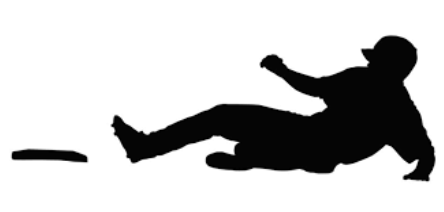
\includegraphics[width=4cm]{documents/figures/2.3-baseball.png}}
\end{center}

\begin{parts}
\part List all forces. Label each as a field or contact force.

\begin{solution}
    \begin{enumerate}
        \item The force on the player by the floor ($F_\text{player-floor}$) and the force on the floor by the player ($F_\text{floor-player}$). These are contact (in the vertical direction) and frictional (in the horizontal) forces.
        \item $F_\text{player-earth}$ and $F_\text{earth-player}$. These are gravitational (field) forces.
        \item $F_\text{floor-earth}$ and $F_\text{earth-floor}$. These are gravitational (field) forces.
    \end{enumerate}
\end{solution}

\part Between what two objects does each force interact?

\begin{solution}
    \begin{enumerate}
        \item $F_\text{player-floor}$ and $F_\text{floor-player}$ interact between the player and floor.
        \item $F_\text{player-earth}$ and $F_\text{earth-player}$ interact between the player and earth.
        \item $F_\text{floor-earth}$ and $F_\text{earth-floor}$ interact between the floor and earth.
    \end{enumerate}
\end{solution}

\part Draw the force pairs and force schema.

\begin{solution}
\phantom{.}

\begin{center}
\begin{tikzpicture}
    \coordinate (earth) at (0,0); 
    \coordinate (floor) at ({4},0); 
    \coordinate (player) at ({4*cos(60)},{4*sin(60)}); 
    \draw (player) node[above] {player};
    \draw (floor) node[right] {floor};
    \draw (earth) node[left] {earth};
    \draw[ultra thick,<->] (player)  -- (floor) node[right=3pt,pos=0.1] {$F_\text{player-floor}$} node[right=3pt,pos=0.8] {$F_\text{floor-player}$};
    \draw[ultra thick,<->] (player) -- (earth) node[left=3pt,pos=0.1] {$F_\text{player-earth}$} node[left=3pt,pos=0.8] {$F_\text{earth-player}$};
    \draw[ultra thick,<->] (earth) -- (floor) node[below=3pt,pos=0.2] {$F_\text{earth-floor}$} node[below=3pt] {$F_\text{floor-earth}$};
\end{tikzpicture}    
\end{center}

\end{solution}
\end{parts}

\clearpage
\begin{EnvUplevel}
    \subsection{Free-Body Diagrams}
\end{EnvUplevel}

\question
An air hockey puck glides across an air hockey table at a constant velocity.

% \begin{center}
%     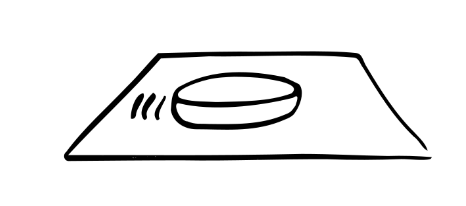
\includegraphics[width=4cm]{documents/figures/2.3-hockey.png}
% \end{center}

\begin{center}
\begin{tikzpicture}
\node[cylinder, 
    draw = black, 
    % text = purple,
    cylinder uses custom fill, 
    cylinder body fill = lightgray, 
    cylinder end fill = gray,
    minimum width = 3cm,
    minimum height = 1cm,
    aspect = 1.5, 
    shape border rotate = 90] (c) at (0,0) {};
\end{tikzpicture}
\end{center}

\begin{parts}
\part Draw the free body diagram.

\begin{solution}
\phantom{.}

\begin{center}
    \begin{tikzpicture}
        \fill (0,0) circle (3pt);
        \draw[ultra thick,->,above=3pt] (0,0) -- ++(0,1.5);
        \draw[ultra thick,->,below=3pt] (0,0) -- ++(0,-1.5);
    \end{tikzpicture}
\end{center}
\end{solution}

\part Are the forces balanced or unbalanced?

\begin{solution}
    Balanced.
\end{solution}

\part Describe the motion, including information about the object's momentum and kinetic energy.

\begin{solution}
    The puck moves at constant velocity, and thus constant momentum and kinetic energy.
\end{solution}

\part Draw a representation of this motion using one of our Multiple Representations. (Recall: Multiple Representations can be position vs time graphs, velocity vs time graphs, momentum vs time graphs, kinetic energy vs time graphs, net force vs time graphs, motion maps.)

\begin{solution}
    \phantom{.}

\begin{center}
\begin{tikzpicture}
    \draw[->] (0,0) -- (0,2) node[above,rotate=90,pos=0.5] {Position};
    \draw[->] (0,0) -- (2,0) node[below,pos=0.5] {Time};
    \draw[ultra thick] (0,0) -- (1.7,1.5);
\end{tikzpicture}
\hspace{1.5ex}
\begin{tikzpicture}
    \draw[->] (0,0) -- (0,2) node[above,rotate=90,pos=0.5] {Velocity};
    \draw[->] (0,0) -- (2,0) node[below,pos=0.5] {Time};
    \draw[ultra thick] (0,1.3) -- ++(1.7,0);
\end{tikzpicture}
\hspace{1.5ex}
\begin{tikzpicture}
    \draw[->] (0,0) -- (0,2) node[above,rotate=90,pos=0.5] {Momentum};
    \draw[->] (0,0) -- (2,0) node[below,pos=0.5] {Time};
    \draw[ultra thick] (0,1.3) -- ++(1.7,0);
\end{tikzpicture}
\hspace{1.5ex}
\begin{tikzpicture}
    \draw[->] (0,0) -- (0,2) node[above,rotate=90,pos=0.5] {Kinetic Energy};
    \draw[->] (0,0) -- (2,0) node[below,pos=0.5] {Time};
    \draw[ultra thick] (0,1.3) -- ++(1.7,0);
\end{tikzpicture}
\hspace{1.5ex}
\begin{tikzpicture}
    \draw[->] (0,0) -- (0,2) node[above,rotate=90,pos=0.5] {Net Force};
    \draw[->] (0,0) -- (2,0) node[below,pos=0.5] {Time};
    \draw[ultra thick] (0,0) -- ++(1.7,0);
\end{tikzpicture}

\vspace{1em}
\begin{tikzpicture}
    \draw[domain=0:5,mark=*,only marks, samples=11] plot(\x,0);
    \draw[thick, ->] (2.5,0.5) -- ++(1,0) node[above,pos=0.5] {$\vec{v}$};
\end{tikzpicture}
\end{center}
\end{solution}
\end{parts}

%*Multiple Representations can be position vs time graphs, velocity vs time graphs, motion maps, momentum vs time graphs, kinetic energy vs time graphs, force vs time graphs.
%**You should choose a different representation for each scenario.

\question
A woman is doing a handstand.

\begin{center}
    
\includegraphics[width=4cm]{documents/figures/2.3-woman.png}
\end{center}

\begin{parts}
\part Draw the free body diagram.

\begin{solution}
\begin{center}
    \begin{tikzpicture}
        \fill (0,0) circle (3pt);
        \draw[ultra thick,->,above=3pt] (0,0) -- ++(0,1.5);
        \draw[ultra thick,->,below=3pt] (0,0) -- ++(0,-1.5);
    \end{tikzpicture}
\end{center}
    
\end{solution}

\part Are the forces balanced or unbalanced?

\begin{solution}
    Balanced.
\end{solution}

\part Describe the motion, including information about the object's momentum and kinetic energy.

\begin{solution}
    The woman is at rest. Her velocity is zero, so her momentum and kinetic energy is zero.
\end{solution}

\part Draw a representation of this motion using one of our Multiple Representations.

\begin{solution}
    \phantom{.}

\begin{center}
\begin{tikzpicture}
    \draw[->] (0,0) -- (0,2) node[above,rotate=90,pos=0.5] {Position};
    \draw[->] (0,0) -- (2,0) node[below,pos=0.5] {Time};
    \draw[ultra thick] (0,1.3) -- ++(1.7,0);
\end{tikzpicture}
\hspace{1.5ex}
\begin{tikzpicture}
    \draw[->] (0,0) -- (0,2) node[above,rotate=90,pos=0.5] {Velocity};
    \draw[->] (0,0) -- (2,0) node[below,pos=0.5] {Time};
    \draw[ultra thick] (0,0) -- ++(1.7,0);
\end{tikzpicture}
\hspace{1.5ex}
\begin{tikzpicture}
    \draw[->] (0,0) -- (0,2) node[above,rotate=90,pos=0.5] {Momentum};
    \draw[->] (0,0) -- (2,0) node[below,pos=0.5] {Time};
    \draw[ultra thick] (0,0) -- ++(1.7,0);
\end{tikzpicture}
\hspace{1.5ex}
\begin{tikzpicture}
    \draw[->] (0,0) -- (0,2) node[above,rotate=90,pos=0.5] {Kinetic Energy};
    \draw[->] (0,0) -- (2,0) node[below,pos=0.5] {Time};
    \draw[ultra thick] (0,0) -- ++(1.7,0);
\end{tikzpicture}
\hspace{1.5ex}
\begin{tikzpicture}
    \draw[->] (0,0) -- (0,2) node[above,rotate=90,pos=0.5] {Net Force};
    \draw[->] (0,0) -- (2,0) node[below,pos=0.5] {Time};
    \draw[ultra thick] (0,0) -- ++(1.7,0);
\end{tikzpicture}

\vspace{1em}
\begin{tikzpicture}
    \fill (0,0) circle (3pt) node[above=4pt] {$\vec{v} = 0$};
\end{tikzpicture}
\end{center}
\end{solution}
\end{parts}

\question
A climber is supported by a rope.

\begin{center}
    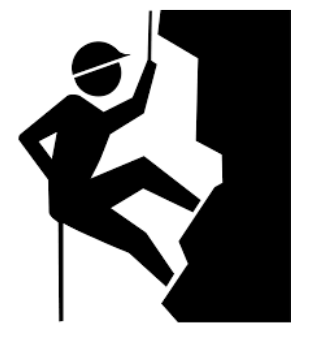
\includegraphics[width=4cm]{documents/figures/2.3-climber.png}
\end{center}

\begin{parts}
\part Draw the free body diagram.

\begin{solution}
\begin{center}
    \begin{tikzpicture}
        \fill (0,0) circle (3pt);
        \draw[ultra thick,->,above=3pt] (0,0) -- ++(0,1.5);
        \draw[ultra thick,->,below=3pt] (0,0) -- ++(0,-1.5);
    \end{tikzpicture}
\end{center}
    
\end{solution}

\part Are the forces balanced or unbalanced?

\begin{solution}
    Balanced.
\end{solution}

\part Describe the motion, including information about the object's momentum and kinetic energy.

\begin{solution}
    The climber is at rest. His velocity is zero, so his momentum and kinetic energy is zero.
\end{solution}

\part Draw a representation of this motion using one of our Multiple Representations.

\begin{solution}
    \phantom{.}

\begin{center}
\begin{tikzpicture}
    \draw[->] (0,0) -- (0,2) node[above,rotate=90,pos=0.5] {Position};
    \draw[->] (0,0) -- (2,0) node[below,pos=0.5] {Time};
    \draw[ultra thick] (0,1.3) -- ++(1.7,0);
\end{tikzpicture}
\hspace{1.5ex}
\begin{tikzpicture}
    \draw[->] (0,0) -- (0,2) node[above,rotate=90,pos=0.5] {Velocity};
    \draw[->] (0,0) -- (2,0) node[below,pos=0.5] {Time};
    \draw[ultra thick] (0,0) -- ++(1.7,0);
\end{tikzpicture}
\hspace{1.5ex}
\begin{tikzpicture}
    \draw[->] (0,0) -- (0,2) node[above,rotate=90,pos=0.5] {Momentum};
    \draw[->] (0,0) -- (2,0) node[below,pos=0.5] {Time};
    \draw[ultra thick] (0,0) -- ++(1.7,0);
\end{tikzpicture}
\hspace{1.5ex}
\begin{tikzpicture}
    \draw[->] (0,0) -- (0,2) node[above,rotate=90,pos=0.5] {Kinetic Energy};
    \draw[->] (0,0) -- (2,0) node[below,pos=0.5] {Time};
    \draw[ultra thick] (0,0) -- ++(1.7,0);
\end{tikzpicture}
\hspace{1.5ex}
\begin{tikzpicture}
    \draw[->] (0,0) -- (0,2) node[above,rotate=90,pos=0.5] {Net Force};
    \draw[->] (0,0) -- (2,0) node[below,pos=0.5] {Time};
    \draw[ultra thick] (0,0) -- ++(1.7,0);
\end{tikzpicture}

\vspace{1em}
\begin{tikzpicture}
    \fill (0,0) circle (3pt) node[above=4pt] {$\vec{v} = 0$};
\end{tikzpicture}
\end{center}
\end{solution}
\end{parts}

\clearpage

\question
A baseball player slows as they slide into the base.

\begin{center}
    \reflectbox{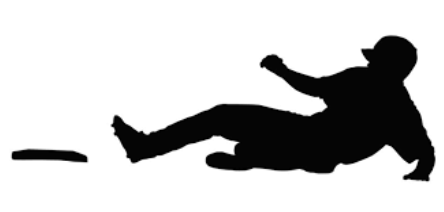
\includegraphics[width=4cm]{documents/figures/2.3-baseball.png}}
\end{center}

\begin{parts}
\part Draw the free body diagram.

\begin{solution}
\begin{center}
    \begin{tikzpicture}
        \fill (0,0) circle (3pt);
        \draw[ultra thick,->,above=3pt] (0,0) -- ++(0,1.5);
        \draw[ultra thick,->,below=3pt] (0,0) -- ++(0,-1.5);
        \draw[ultra thick,->,right=3pt] (0,0) -- ++(-1,0) node[left] {\small friction};
    \end{tikzpicture}
\end{center}
    
\end{solution}

\part Are the forces balanced or unbalanced?

\begin{solution}
    The vertical forces are balanced. In the horizontal direction, the frictional force is unbalanced and slows the player down.
\end{solution}

\part Describe the motion, including information about the object's momentum and kinetic energy.

\begin{solution}
    The player is moving to the right and is impacted by a leftward frictional force that slows him down. He has decreasing momentum and decreasing kinetic energy.
\end{solution}

\part Draw a representation of this motion using one of our Multiple Representations.

\begin{solution}
    The only representations that may be intuitive to students is net force vs time graph and the motion map:

\begin{center}
\begin{tikzpicture}
    \draw[->] (0,-1) -- (0,1) node[above,rotate=90,pos=0.5] {Net Force};
    \draw[->] (0,0) -- ++(2,0) node[right,] {Time};
    \draw[ultra thick] (0,-0.5) -- ++(1.7,0);
\end{tikzpicture}

\vspace{5mm}

\begin{tikzpicture}[scale=0.6]
    \draw[domain=-10:0,mark=*,only marks, samples=6,mark size=3.5pt] plot({0.1*\x^2},0);
    \draw[thick, <-] (-5,0.5) -- ++(-1,0) node[above,pos=0.5] {$\vec{v}$};
\end{tikzpicture}
\end{center}

\vspace{5mm}

The remaining representations are

\begin{center}
    \begin{tikzpicture}
        \begin{axis}[height=4cm,
            width=4cm,
            ymin=0,ymax=7,
            xmin=0,xmax=3,
            ticks=none,
            axis lines=left,
            ylabel={Position},
            xlabel={Time},
        ]
            \addplot[domain=0:2.5,ultra thick,black] {5*x - (100/(2*50))*x^2};
        \end{axis}
    \end{tikzpicture}
    \hspace{1em}
    \begin{tikzpicture}
        \begin{axis}[height=4cm,
            width=4cm,
            ymin=0,ymax=6,
            xmin=0,xmax=3,
            ticks=none,
            axis lines=left,
            ylabel={Velocity},
            xlabel={Time},
        ]
            \addplot[domain=0:2.5,ultra thick,black] {5 - 100/50*x};
        \end{axis}
    \end{tikzpicture}
    \hspace{1em}
    \begin{tikzpicture}
        \begin{axis}[height=4cm,
            width=4cm,
            ymin=0,ymax=300,
            xmin=0,xmax=3,
            ticks=none,
            axis lines=left,
            ylabel={Momentum},
            xlabel={Time},
        ]
            \addplot[domain=0:2.5,ultra thick,black] {50*5 - 100*x};
        \end{axis}
    \end{tikzpicture}
    \hspace{1em}
    \begin{tikzpicture}
        \begin{axis}[height=4cm,
            width=4cm,
            ymin=0,ymax=700,
            xmin=0,xmax=3,
            ticks=none,
            axis lines=left,
            ylabel={Kinetic Energy},
            xlabel={Time},
        ]
            \addplot[domain=0:2.5,ultra thick,black] {0.5*50*(5 - 100*x/50)^2};
        \end{axis}
    \end{tikzpicture}
\end{center}


and the proof is below.

For the purpose of demonstration, let's make up some numbers. The player's mass is $m=\SI{50}{kg}$, his initial velocity is $v_0 = +\SI{5}{m/s}$, and he is subject to a frictional force of magnitude $f = \SI{100}{N}$ in the negative (leftward) direction. By Newton's second law the player's acceleration is

\begin{equation*}
    a = -\frac{f}{m} = \SI{-2}{m/s^2}
\end{equation*}

Assuming he starts at $x_0 = 0$, his position as a function of time is

\begin{equation*}
    x(t) = v_0 t + \frac{1}{2}a t^2 = v_0 t -\left(\frac{f}{2m}\right)t^2
\end{equation*}

and is graphed below.

\begin{center}
    \begin{tikzpicture}
        \begin{axis}[height=6cm,
            width=6cm,
            ymin=0,ymax=7,
            xmin=0,xmax=3,
            ytick={0,1,...,7},
            xtick={0,0.5,...,3},
            axis lines=left,
            ylabel={Position (m)},
            xlabel={Time (s)},
            grid=both,
        ]
            \addplot[domain=0:2.5,ultra thick,black] {5*x - (100/(2*50))*x^2};
        \end{axis}
    \end{tikzpicture}
\end{center}

The player's velocity as a function of time is given by

\begin{equation*}
    v(t) = v_0 + a t = v_0 - \frac{ft}{m} 
\end{equation*}

and is graphed below.

\begin{center}
    \begin{tikzpicture}
        \begin{axis}[height=6cm,
            width=6cm,
            ymin=0,ymax=6,
            xmin=0,xmax=3,
            ytick={0,1,...,6},
            xtick={0,0.5,...,3},
            axis lines=left,
            ylabel={Velocity (m/s)},
            xlabel={Time (s)},
            grid=both,
        ]
            \addplot[domain=0:2.5,ultra thick,black] {5 - 100/50*x};
        \end{axis}
    \end{tikzpicture}
\end{center}

His momentum is

\begin{equation*}
    p = m v(t) = mv_0 - ft
\end{equation*}

and is graphed below.

\begin{center}
    \begin{tikzpicture}
        \begin{axis}[height=6cm,
            width=6cm,
            ymin=0,ymax=300,
            xmin=0,xmax=3,
            ytick={0,50,...,300},
            xtick={0,0.5,...,3},
            axis lines=left,
            ylabel={Momentum (\SI{}{kg\cdot m/s})},
            xlabel={Time (s)},
            grid=both,
        ]
            \addplot[domain=0:2.5,ultra thick,black] {50*5 - 100*x};
        \end{axis}
    \end{tikzpicture}
\end{center}


His kinetic energy as a function of time is

\begin{align*}
    \mathrm{KE}(t) &= \frac{1}{2} m \left[v(t)\right]^2 \\[1em]
        &= \frac{1}{2} m \left(v_0 - \frac{ft}{m}\right)^2 \\[1em]
        &= \frac{1}{2} m v_0^2 - fv_0 t + \left(\frac{f^2}{2m}\right) t^2
\end{align*}

and is graphed below:

\begin{center}
    \begin{tikzpicture}
        \begin{axis}[height=6cm,
            width=6cm,
            ymin=0,ymax=700,
            xmin=0,xmax=3,
            ytick={0,100,...,700},
            xtick={0,0.5,...,3},
            axis lines=left,
            ylabel={Kinetic Energy (J)},
            xlabel={Time (s)},
            grid=both,
        ]
            \addplot[domain=0:2.5,ultra thick,black] {0.5*50*(5 - 100*x/50)^2};
        \end{axis}
    \end{tikzpicture}
\end{center}
\end{solution}
\end{parts}

\clearpage
\begin{EnvUplevel}
    \subsection{Balanced and Unbalanced Forces (Part I)}

    \textbf{Questions \ref{cTXNT}--\ref{HPDAU}.} Access the PhET Simulation: Forces and Motion (\href{https://phet.colorado.edu/sims/html/forces-and-motion-basics/latest/forces-and-motion-basics_all.html}{CLICK HERE}).

    \textbf{PART 1: TUG OF WAR.} 
    
    Make sure all boxes (Force, Sum of Forces, Values, Masses, Speed) in the upper right hand corner are checked.
\end{EnvUplevel}

\question \label{cTXNT}
Create a scenario in which the forces are balanced. Draw a picture of the vector arrows and the net force (sum of forces). What is the net force on the cart? 

\begin{solution}
\begin{center}
\begin{tikzpicture}
    \fill (0,0) circle (5pt);
    \draw[thick,->] (0,0) -- (3,0) node[right] {100\,N};
    \draw[thick,->] (0,0) -- (-3,0) node[left] {100\,N};
\end{tikzpicture}

\begin{equation*}
    F_\mathrm{net} = 0
\end{equation*}
\end{center}
\end{solution}

\question
Create a scenario in which the forces are unbalanced. Draw a picture of the vector arrows and the net force (sum of forces). What is the net force on the cart?

\begin{solution}
\begin{center}
\begin{tikzpicture}
    \fill (0,0) circle (5pt);
    \draw[thick,->] (0,0) -- ({3*1.5},0) node[right] {150\,N};
    \draw[thick,->] (0,0) -- (-3,0) node[left] {100\,N};
\end{tikzpicture}

\begin{equation*}
    F_\mathrm{net} = \SI{100}{N} - \SI{50}{N} = \SI{50}{N}
\end{equation*}

\end{center}
\end{solution}


\begin{EnvUplevel}
    \textbf{PART 2: MOTION.} 
    
    Click the Motion Panel. Make sure all boxes (Force, Sum of Forces, Values, Masses, Speed) in the upper right hand corner are checked. Note: There is no friction in this scenario.
\end{EnvUplevel}

\question
Place the refrigerator on the skateboard. Apply a force of 100\,N. Once the skateboard is moving, set the force to 0 Newtons (which represents letting go). 

\begin{parts}
    \part What happens to the speed of the skateboard-refrigerator system when there is no longer a force being applied?

    \begin{solution}
        Speed stays constant.
    \end{solution}
    
    \part Are the forces acting on the skateboard-refrigerator balanced or unbalanced?

    \begin{solution}
        Balanced.
    \end{solution}
    
    \part What are the forces acting on the skateboard-refrigerator system?

    \begin{solution}
        None in the horizontal direction. In the vertical direction, the force of gravity and the normal force.
    \end{solution}
    
    \part Will the skateboard-refrigerator system ever stop moving? Why or why not explain?

    \begin{solution}
        No. According to Newton's first law (the law of inertia), an object in motion will stay in motion at a constant velocity unless acted on by a net external force.
    \end{solution}
\end{parts}

\question
Reset the simulation and click all boxes again. Place the refrigerator on the skateboard and apply a force of 100\,N. This time, do not stop applying the force to the skateboard-refrigerator system. 

\begin{parts}
    \part What happens to the speed of the skateboard-refrigerator system when the force is continuously applied?

    \begin{solution}
        The speed increases over time.
    \end{solution}
    
    \part Are the forces acting on the skateboard-refrigerator system balanced or unbalanced?

    \begin{solution}
        The forces are unbalanced because now there's a net force in the horizontal direction.
    \end{solution}
    
    \part Will the speed of the skateboard-refrigerator system ever stop changing? Why or why not?

    \begin{solution}
        No. The speed will continue to increase as long as the forces are unbalanced.
    \end{solution}
\end{parts}

\begin{EnvUplevel}
    \textbf{PART 3: FRICTION.}

    Click on the Friction panel. Make sure all boxes (Force, Sum of Forces, Values, Masses, Speed) in the upper right hand corner are checked. Do not change the magnitude of friction.
\end{EnvUplevel}

\question
How does the presence of friction affect the movement of the objects in the simulation?

\begin{solution}
    Friction opposes the applied force and causes objects in motion to slow down and eventually stop.
\end{solution}

\question
Before the object starts moving, what do you notice about the frictional force and the applied force? Are the forces balanced or unbalanced?

\begin{solution}
    Friction is equal in magnitude to the applied force.
\end{solution}

\question 
After the object starts moving, what do you notice about the friction force and the applied force? Are the forces balanced or unbalanced?

\begin{solution}
    The applied force is greater in magnitude than the friction force.
\end{solution}

\question
Place one 50\,kg box on the ground. What is the minimum amount of force required to get the box moving?

\begin{solution}
    126\,N
\end{solution}

\question
Place the second 50\,kg box on top of the first. Predict the minimum amount of force that will be required to get the box moving.

\begin{solution}
    251\,N
\end{solution}

\question
What is the minimum amount of force required to get the 2-box (100\,kg) system of boxes moving?

\begin{solution}
    251\,N
\end{solution}

\question
How are these two forces related?

\begin{solution}
    The forces increase with increasing mass. 
\end{solution}

\question
Predict how much force is required to move the refrigerator.

\begin{solution}
    500\,N
\end{solution}

\question \label{HPDAU}
What is the mass of the present? Explain how you got your answer.



\clearpage

\begin{EnvUplevel}
    \textbf{Questions .} \textit{Ball \& Broom Activity.} We will be applying a constant force to a bowling ball with a broom. Then we will analyze the motion of the ball and the forces involved. We will be able to draw a Free Body Diagram (FBD) of a situation. Additionally, be able to predict the motion and changes in motion and whether the forces are balanced or unbalanced based on a FBD.
\end{EnvUplevel}

\question
Scenario 1. Place the bowling ball on the floor. Do not push on the ball with anything.

\begin{parts}
    \part Draw a Motion Map of the bowling ball.
    \part Draw a Free Body Diagram of the bowling ball.
    \part Were the forces acting on the bowling ball balanced or unbalanced?
    \part Describe the motion of the object.
\end{parts}

\question
Scenario 2.

\begin{itemize}[itemsep=0pt,topsep=0pt]
    \item Student A should gently push the ball with his/her foot/hand so that it just barely begins moving.
    \item Student B should say ``drop'' every 2 seconds until the ball reaches the end of the path.
    \item Student C should drop the coin next to the bowling ball each time Student B says ``drop.''
\end{itemize}

\medskip

\begin{parts}
    \part Draw a Motion Map of the bowling ball.
    \part Draw a Free Body Diagram of the bowling ball.
    \part Were the forces acting on the bowling ball balanced or unbalanced?
    \part Describe the motion of the object.
\end{parts}

\question 
Scenario 3.

\begin{itemize}[itemsep=0pt,topsep=0pt]
    \item Student A should gently push the ball with his/her foot/hand so that it just barely begins moving.
    \item Student A just barely pushes on the ball with the broom with a force just barely large enough to keep the ball moving to the end of the path. The force should be kept constant, so try not to push less or more at different points.  The broom should be kept on the ball the entire time.
    \item Student B should say ``drop'' every 2 seconds until the ball reaches the end of the path.
    \item Student C should drop the coin next to the bowling ball each time Student B says ``drop.''
\end{itemize}

\medskip

\begin{parts}
    \part Draw a Motion Map of the bowling ball.
    \part Draw a Free Body Diagram of the bowling ball.
    \part Were the forces acting on the bowling ball balanced or unbalanced?
    \part Describe the motion of the object.
\end{parts}

\question
In which scenario(s) were the forces balanced?

\begin{solution}
    Scenarios 1 and 2.
\end{solution}

\question
In which scenario(s) was the ball's velocity changing?

\begin{solution}
    Scenario 3.
\end{solution}

\question
Newton’s Law of Inertia is traditionally written as ``An object at rest stays at rest and an object in motion stays in motion unless acted upon by an unbalanced force.'' 

\begin{parts}
    \part How did the above activity show evidence for that law?

    \begin{solution}
        Scenario 1 shown the bowling ball staying at rest, and Scenario 2 showed it remaining in motion. Scenario 3 shown the unbalanced force changing the ball's velocity.
    \end{solution}
    
    \part Based on the activity and class discussion, rewrite Newton's Law of Inertia in your own words.

    \begin{solution}
        Answers may vary.
    \end{solution}
\end{parts}

\clearpage
\begin{multicols*}{2}


\question \label{T7nyj}
The object below is moving to the right.

\begin{center}
    \begin{tikzpicture}
        \fill (0,0) circle (3pt);
        \draw[ultra thick,<->] (0,-1) -- (0,1);
    \end{tikzpicture}
\end{center}

The object is\dots .

\begin{randomizechoices}[norandomize]
    \choice speeding up
    \choice slowing down
    \correctchoice moving at constant speed 
\end{randomizechoices}

\question \label{lUN3c}
Are the force on the object balanced or unbalanced?

\begin{randomizechoices}[norandomize]
    \correctchoice balanced
    \choice unbalanced
\end{randomizechoices}

\bigskip
\hrule

\question \label{CrTRg}
The object below is moving to the left.


\begin{center}
    \begin{tikzpicture}
        \fill (0,0) circle (3pt);
        \draw[ultra thick,<->] (0,-1) -- (0,1);
        \draw[ultra thick,->] (0,0) -- (1,0);
    \end{tikzpicture}
\end{center}

The object is\dots .

\begin{randomizechoices}[norandomize]
    \choice speeding up
    \correctchoice slowing down
    \choice moving at constant speed 
\end{randomizechoices}

\question \label{TzyfS}
Are the force on the object balanced or unbalanced?

\begin{randomizechoices}[norandomize]
    \choice balanced
    \correctchoice unbalanced
\end{randomizechoices}

\bigskip
\hrule


\question \label{ayuwJ}
The object below is moving to the left.

\begin{center}
    \begin{tikzpicture}
        \fill (0,0) circle (3pt);
        \draw[ultra thick,<->] (0,-1) -- (0,1);
        \draw[ultra thick,<->] (-1,0) -- (1,0);
    \end{tikzpicture}
\end{center}

The object is\dots .

\begin{randomizechoices}[norandomize]
    \choice speeding up
    \choice slowing down
    \correctchoice moving at constant speed 
\end{randomizechoices}

\question \label{vYsXn}
Are the force on the object balanced or unbalanced?

\begin{randomizechoices}[norandomize]
    \correctchoice balanced
    \choice unbalanced
\end{randomizechoices}

\bigskip
\hrule



\vspace*{\fill}
\columnbreak


\question 
The object below is moving to the right.

\begin{center}
    \begin{tikzpicture}
        \fill (0,0) circle (3pt);
        \draw[ultra thick,<->] (0,-1) -- (0,1);
        \draw[ultra thick,<->] (-2,0) -- (1,0);
    \end{tikzpicture}
\end{center}

The object is\dots .

\begin{randomizechoices}[norandomize]
    \choice speeding up
    \correctchoice slowing down
    \choice moving at constant speed 
\end{randomizechoices}

\question 
Are the force on the object balanced or unbalanced?

\begin{randomizechoices}[norandomize]
    \choice balanced
    \correctchoice unbalanced
\end{randomizechoices}

\bigskip
\hrule

\question
The object below is moving to the down.

\begin{center}
    \begin{tikzpicture}
        \fill (0,0.4) circle (3pt);
        \draw[ultra thick,<->] (0,-1) -- (0,1);
    \end{tikzpicture}
\end{center}

The object is\dots .

\begin{randomizechoices}[norandomize]
    \correctchoice speeding up
    \choice slowing down
    \choice moving at constant speed 
\end{randomizechoices}

\question 
Are the force on the object balanced or unbalanced?

\begin{randomizechoices}[norandomize]
    \choice balanced
    \correctchoice unbalanced
\end{randomizechoices}

\bigskip
\hrule

\question 
The object below is moving to the right.

\begin{center}
    \begin{tikzpicture}
        \fill (0,0) circle (3pt);
        \draw[ultra thick,<->] (0,-0.7) -- (0,0.7);
        \draw[ultra thick,<->] (-1,0) -- (2,0);
    \end{tikzpicture}
\end{center}

The object is\dots .

\begin{randomizechoices}[norandomize]
    \correctchoice speeding up
    \choice slowing down
    \choice moving at constant speed 
\end{randomizechoices}

\question 
Are the force on the object balanced or unbalanced?

\begin{randomizechoices}[norandomize]
    \choice balanced
    \correctchoice unbalanced
\end{randomizechoices}

\bigskip
\hrule

\vspace*{\fill}
\end{multicols*}

\question
The graph depicts the motion of an object.

\begin{center}
    \begin{tikzpicture}
        \begin{axis}[height=5cm,width=5cm,
            axis lines=left,
            ymin=0,ymax=10,
            xmin=0,xmax=10,
            ylabel={Position},
            xlabel={Time},
            xtick=\empty,
            ytick=\empty,
            clip=false,
        ]
        \addplot[ultra thick,black,domain=1:9] {8/x^0.8};
        \end{axis}
    \end{tikzpicture}
\end{center}

\begin{parts}
\part Is the object speeding up, slowing down, or moving at constant speed?

\begin{solution}
    Slowing down.
\end{solution}

\part Are the forces on the object balanced or unbalanced?

\begin{solution}
    Unbalanced.
\end{solution}
\end{parts}

\question
The graph depicts the motion of an object. 

\begin{center}
    \begin{tikzpicture}
        \begin{axis}[height=5cm,width=5cm,
            axis lines=left,
            ymin=0,ymax=10,
            xmin=0,xmax=10,
            ylabel={Position},
            xlabel={Time},
            xtick=\empty,
            ytick=\empty,
            clip=false,
        ]
        \addplot[ultra thick,black,domain=0:8] {x};
        \end{axis}
    \end{tikzpicture}
\end{center}

\begin{parts}
    \part Is the object speeding up, slowing down, or moving at constant speed?

\begin{solution}
    Moving at constant speed.
\end{solution}

    \part Are the forces on the object balanced or unbalanced?

\begin{solution}
    Balanced.
\end{solution}
\end{parts}


\question
The graph depicts the motion of an object. 

\begin{center}
    \begin{tikzpicture}
        \begin{axis}[height=5cm,width=5cm,
            axis lines=left,
            ymin=0,ymax=10,
            xmin=0,xmax=10,
            ylabel={Position},
            xlabel={Time},
            xtick=\empty,
            ytick=\empty,
            clip=false,
        ]
        \addplot[ultra thick,black,domain=0:8] {-1*x+8};
        \end{axis}
    \end{tikzpicture}
\end{center}

\begin{parts}
\part Is the object speeding up, slowing down, or moving at constant speed?

\begin{solution}
    Moving at constant speed.
\end{solution}

\part Are the forces on the object balanced or unbalanced?

\begin{solution}
    Balanced.
\end{solution}
\end{parts}

\clearpage
\question
The graph depicts the motion of an object.

\begin{center}
\begin{tikzpicture}
    \begin{axis}[height=5cm,
        width=5cm,
        ymin=0,ymax=7,
        xmin=0,xmax=3,
        ticks=none,
        axis lines=left,
        ylabel={Position},
        xlabel={Time},
    ]
        \addplot[domain=0:2.5,ultra thick,black] {5*x - (100/(2*50))*x^2};
    \end{axis}
\end{tikzpicture}    
\end{center}

\begin{parts}
\part Is the object speeding up, slowing down, or moving at constant speed?

\begin{solution}
    Slowing down.
\end{solution}

\part Are the forces on the object balanced or unbalanced?

\begin{solution}
    Unbalanced.
\end{solution}
\end{parts}

\question
Consider the motion map below. The arrow indicates the object's velocity.

\begin{center}
    \begin{tikzpicture}
        \draw[domain=0:10,mark=*,only marks, samples=11] plot(\x,0);
        \draw[thick, ->] (4,0.5) -- ++(1,0) node[above,pos=0.5] {$\vec{v}$};
    \end{tikzpicture}
\end{center}

\begin{parts}
\part Is the object speeding up, slowing down, or moving at constant speed?

\begin{solution}
    Moving at constant speed.
\end{solution}

\part Are the forces on the object balanced or unbalanced?

\begin{solution}
    Unbalanced.
\end{solution}
\end{parts}


\question
Consider the motion map below. The arrow indicates the object's velocity.

\begin{center}
    \begin{tikzpicture}
        \draw[domain=0:10,mark=*,only marks, samples=6] plot({0.1*\x^2},0);
        \draw[thick, <-] (5,0.5) -- ++(-1,0) node[above,pos=0.5] {$\vec{v}$};
    \end{tikzpicture}
\end{center}

\begin{parts}
\part Is the object speeding up, slowing down, or moving at constant speed?

\begin{solution}
    Speeding up.
\end{solution}

\part Are the forces on the object balanced or unbalanced?

\begin{solution}
    Unbalanced.
\end{solution}
\end{parts}

\question
Consider the motion map below. The arrow indicates the object's velocity.

\begin{center}
    \begin{tikzpicture}
        \draw[domain=0:10,mark=*,only marks, samples=6] plot({0.1*\x^2},0);
        \draw[thick, ->] (5,0.5) -- ++(-1,0) node[above,pos=0.5] {$\vec{v}$};
    \end{tikzpicture}
\end{center}

\begin{parts}
\part Is the object speeding up, slowing down, or moving at constant speed?

\begin{solution}
    Slowing down.
\end{solution}

\part Are the forces on the object balanced or unbalanced?

\begin{solution}
    Slowing down.
\end{solution}

\end{parts}

\question
Consider the motion map below. The arrow indicates the object's velocity.

\begin{center}
    \begin{tikzpicture}
        \draw[domain=0:10,mark=*,only marks, samples=11] plot(\x,0);
        \draw[thick, <-] (4,0.5) -- ++(1,0) node[above,pos=0.5] {$\vec{v}$};
    \end{tikzpicture}
\end{center}

\begin{parts}
\part Is the object speeding up, slowing down, or moving at constant speed?

\begin{solution}
    Moving at constant speed.
\end{solution}

\part Are the forces on the object balanced or unbalanced?

\begin{solution}
    Balanced.
\end{solution}
\end{parts}

\clearpage
\question
The graph depicts the motion of an object.

\begin{center}
    \begin{tikzpicture}
        \begin{axis}[height=5cm,width=5cm,
            axis y line=left,
            axis x line=center,
            ymin=-5,ymax=5,
            xmin=0,xmax=10,
            ylabel={Velocity},
            xlabel={Time},
            xtick=\empty,
            ytick=\empty,
            clip=false,
            x label style={at={(axis description cs: 1,0.5)},anchor=west}
        ]
        \addplot[ultra thick,black,domain=0:8] {0.5*x};
        \end{axis}
    \end{tikzpicture}
\end{center}

\begin{parts}
\part Is the object speeding up, slowing down, or moving at constant speed?

\begin{solution}
    Speeding up.
\end{solution}

\part Are the forces on the object balanced or unbalanced?

\begin{solution}
    Unbalanced.
\end{solution}
\end{parts}

\question
The graph depicts the motion of an object.

\begin{center}
    \begin{tikzpicture}
        \begin{axis}[height=5cm,width=5cm,
            axis y line=left,
            axis x line=center,
            ymin=-5,ymax=5,
            xmin=0,xmax=10,
            ylabel={Velocity},
            xlabel={Time},
            xtick=\empty,
            ytick=\empty,
            clip=false,
            x label style={at={(axis description cs: 1,0.5)},anchor=west}
        ]
        \addplot[ultra thick,black,domain=0:9] {-2.5};
        \end{axis}
    \end{tikzpicture}
\end{center}

\begin{parts}
\part Is the object speeding up, slowing down, or moving at constant speed?

\begin{solution}
    Moving at constant speed.
\end{solution}

\part Are the forces on the object balanced or unbalanced?

\begin{solution}
    Balanced.
\end{solution}
\end{parts}

\question
The table below depicts the motion of an object.

\begin{center}
    \begin{tabular}{|c|c|}
        \hline
        \textbf{Time} (s) & \textbf{Velocity} (m/s) \\ \hline
        $0$ & $-0$ \\ \hline 
        $1$ & $-3$ \\ \hline
        $2$ & $-6$ \\ \hline
        $3$ & $-9$ \\ \hline
        $4$ & $-12$ \\ \hline
        $5$ & $-15$ \\ \hline
    \end{tabular}
\end{center}

\begin{parts}
\part Is the object speeding up, slowing down, or moving at constant speed?

\begin{solution}
    Speeding up.
\end{solution}

\part Are the forces on the object balanced or unbalanced?

\begin{solution}
    Unbalanced.
\end{solution}
\end{parts}

\question
The table below depicts the motion of an object.

\begin{center}
    \begin{tabular}{|c|c|}
        \hline
        \textbf{Time} (s) & \textbf{Position} (m) \\ \hline
        $0$ & $25$ \\ \hline 
        $1$ & $20$ \\ \hline
        $2$ & $15$ \\ \hline
        $3$ & $10$ \\ \hline
        $4$ & $5$ \\ \hline
        $5$ & $0$ \\ \hline
    \end{tabular}
\end{center}

\begin{parts}
\part Is the object speeding up, slowing down, or moving at constant speed?


\begin{solution}
    Moving at constant speed.
\end{solution}

\part Are the forces on the object balanced or unbalanced?

\begin{solution}
    Balanced.
\end{solution}
\end{parts}

\clearpage
\question
The table below depicts the motion of an object.

\begin{center}
    \begin{tabular}{|c|c|}
        \hline
        \textbf{Time} (s) & \textbf{Position} (m) \\ \hline
        $0$ & $0$ \\ \hline 
        $1$ & $15$ \\ \hline
        $2$ & $27$ \\ \hline
        $3$ & $36$ \\ \hline
        $4$ & $42$ \\ \hline
        $5$ & $45$ \\ \hline
    \end{tabular}
\end{center}

\begin{parts}
\part Is the object speeding up, slowing down, or moving at constant speed?

\begin{solution}
    Slowing down.
\end{solution}

\part Are the forces on the object balanced or unbalanced?

\begin{solution}
    Unbalanced.
\end{solution}
\end{parts}


\clearpage
\begin{EnvUplevel}
    \subsection{Balanced Forces (Part II): Quiz a Friend Activity}
\end{EnvUplevel}

\question
A force is required to keep an object moving in a given direction.

\begin{randomizechoices}[norandomize]
    \choice True
    \correctchoice False
\end{randomizechoices}

\question
If an object is at rest, then there are no forces acting upon the object.

\begin{randomizechoices}[norandomize]
    \choice True
    \correctchoice False
\end{randomizechoices}

\question
An unbalanced force means that an object's kinetic energy and momentum are changing.

\begin{randomizechoices}[norandomize]
    \correctchoice True
    \choice False
\end{randomizechoices}

\question
An object whose forces are balanced will not have momentum or kinetic energy.

\begin{randomizechoices}[norandomize]
    \choice True
    \correctchoice False
\end{randomizechoices}

\question
An object's inertia is only important if the object is not moving.

\begin{randomizechoices}[norandomize]
    \choice True
    \correctchoice False
\end{randomizechoices}

\clearpage

 
    

\question
Quiz A Friend Activity.

\fbox{
\begin{minipage}[c][4cm][c]{0.45\textwidth}
\centering
    \begin{tabular}{|c|c|}
        \hline
        \textbf{Time} (s) & \textbf{Velocity} (m/s) \\ \hline
        $0$ & $0$ \\ \hline 
        $1$ & $4$ \\ \hline
        $2$ & $8$ \\ \hline
        $3$ & $12$ \\ \hline
        $4$ & $16$ \\ \hline
    \end{tabular}     .
\end{minipage}
}%
\fbox{
\begin{minipage}[c][4cm][c]{0.45\textwidth}
\centering
    \begin{itemize}[itemsep=0pt]
        \item Changing Velocity
        \item Unbalanced Forces
        \item Changing Momentum
        \item Changing Kinetic Energy
        \item Speeding up away from the reference point
    \end{itemize}   .
\end{minipage}
}

\fbox{
\begin{minipage}[c][4cm][c]{0.45\textwidth}
\centering
    \begin{tikzpicture}
        \fill (0,0) circle (3pt);
        \draw[ultra thick,<->] (0,-1) -- (0,1);
        \draw[ultra thick,<->] (-1,0) -- (1,0);
    \end{tikzpicture}
\end{minipage}
}%
\fbox{
\begin{minipage}[c][4cm][c]{0.45\textwidth}
\centering
    \begin{itemize}[itemsep=0pt]
        \item At rest or moving with a constant velocity
        \item Balanced Forces
        \item No or constant momentum
        \item No or constant kinetic energy
    \end{itemize}
\end{minipage}
}

\fbox{
\begin{minipage}[c][4cm][c]{0.45\textwidth}
\centering
    \begin{tikzpicture}
        \begin{axis}[height=5cm,width=5cm,
            axis y line=left,
            axis x line=center,
            ymin=-5,ymax=5,
            xmin=0,xmax=10,
            ylabel={Velocity},
            xlabel={Time},
            xtick=\empty,
            ytick=\empty,
            clip=false,
            x label style={at={(axis description cs: 1,0.5)},anchor=west}
        ]
        \addplot[ultra thick,black,domain=0:8] {0.5*x};
        \end{axis}
    \end{tikzpicture}
\end{minipage}
}%
\fbox{
\begin{minipage}[c][4cm][c]{0.45\textwidth}
\centering
    \begin{itemize}[itemsep=0pt]
        \item Changing velocity
        \item Unbalanced Forces
        \item Speeding up away from the reference point.
        \item Changing Momentum
        \item Changing Kinetic Energy
    \end{itemize}
\end{minipage}
}

\fbox{
\begin{minipage}[c][4cm][c]{0.45\textwidth}
\centering
\begin{center}
    \begin{tikzpicture}[scale=0.6]
        \draw[domain=0:10,mark=*,only marks, samples=6,mark size=3.5pt] plot({0.1*\x^2},0);
        \draw[thick, <-] (5,0.5) -- ++(-1,0) node[above,pos=0.5] {$\vec{v}$};
    \end{tikzpicture}
\end{center}

\end{minipage}
}%
\fbox{
\begin{minipage}[c][4cm][c]{0.45\textwidth}
\centering
    \begin{itemize}[itemsep=0pt]
        \item Changing velocity
        \item Unbalanced forces
        \item Speeding up away from the reference point.
        \item Changing Momentum
        \item Changing Kinetic Energy
    \end{itemize}
\end{minipage}
}

\fbox{
\begin{minipage}[c][4cm][c]{0.45\textwidth}
\centering
    \begin{tikzpicture}
        \fill (0,0) circle (3pt);
        \draw[ultra thick,<->] (0,-1) -- (0,1);
        \draw[ultra thick,->] (0,0) -- (1,0);
    \end{tikzpicture}
\end{minipage}
}%
\fbox{
\begin{minipage}[c][4cm][c]{0.45\textwidth}
\centering
    \begin{itemize}[itemsep=0pt]
        \item Unbalanced forces
        \item Changing velocity
        \item Speeding up to the right or slowing down to the left.
        \item Changing Momentum
        \item Changing Kinetic Energy
    \end{itemize}
\end{minipage}
}

\fbox{
\begin{minipage}[c][4cm][c]{0.45\textwidth}
\centering
    \begin{tikzpicture}
        \begin{axis}[height=5cm,width=5cm,
            axis y line=left,
            axis x line=center,
            ymin=-5,ymax=5,
            xmin=0,xmax=10,
            ylabel={Velocity},
            xlabel={Time},
            xtick=\empty,
            ytick=\empty,
            clip=false,
            x label style={at={(axis description cs: 1,0.5)},anchor=west}
        ]
        \addplot[ultra thick,black,domain=0:8] {4-0.5*x};
        \end{axis}
    \end{tikzpicture}
\end{minipage}
}%
\fbox{
\begin{minipage}[c][4cm][c]{0.45\textwidth}
\centering
    \begin{itemize}[itemsep=0pt]
        \item Changing velocity
        \item Unbalanced Forces
        \item Changing Momentum
        \item Changing kinetic energy
        \item Slowing down towards the reference point
    \end{itemize}
\end{minipage}
}

\fbox{
\begin{minipage}[c][4cm][c]{0.45\textwidth}
\centering
    \begin{tikzpicture}
        \begin{axis}[height=5cm,width=5cm,
            axis y line=left,
            axis x line=center,
            ymin=-5,ymax=5,
            xmin=0,xmax=10,
            ylabel={Velocity},
            xlabel={Time},
            xtick=\empty,
            ytick=\empty,
            clip=false,
            x label style={at={(axis description cs: 1,0.5)},anchor=west}
        ]
        \addplot[ultra thick,black,domain=0:8] {3};
        \end{axis}
    \end{tikzpicture}
\end{minipage}
}%
\fbox{
\begin{minipage}[c][4cm][c]{0.45\textwidth}
\centering
    \begin{itemize}[itemsep=0pt]
        \item Constant Velocity
        \item Balanced Forces
        \item Constant Momentum
        \item Constant Kinetic Energy
        \item Moving away from the reference point
    \end{itemize}
\end{minipage}
}

\fbox{
\begin{minipage}[c][4cm][c]{0.45\textwidth}
\centering
    \begin{tikzpicture}
        \begin{axis}[height=5cm,width=5cm,
            axis y line=left,
            axis x line=center,
            ymin=-5,ymax=5,
            xmin=0,xmax=10,
            ylabel={Velocity},
            xlabel={Time},
            xtick=\empty,
            ytick=\empty,
            clip=false,
            x label style={at={(axis description cs: 1,0.5)},anchor=west}
        ]
        \addplot[ultra thick,black,domain=0:8] {-3};
        \end{axis}
    \end{tikzpicture}
\end{minipage}
}%
\fbox{
\begin{minipage}[c][4cm][c]{0.45\textwidth}
\centering
    \begin{itemize}[itemsep=0pt]
        \item Constant Velocity
        \item Balanced Forces
        \item Constant Momentum
        \item Constant Kinetic Energy
        \item Moving towards the reference point
    \end{itemize}
\end{minipage}
}

\fbox{
\begin{minipage}[c][4cm][c]{0.45\textwidth}
\centering
    \begin{tikzpicture}
        \begin{axis}[height=5cm,width=5cm,
            axis lines=left,
            ymin=0,ymax=10,
            xmin=0,xmax=10,
            ylabel={Position},
            xlabel={Time},
            xtick=\empty,
            ytick=\empty,
            clip=false,
        ]
        \addplot[ultra thick,black,domain=0:8] {-1*x+8};
        \end{axis}
    \end{tikzpicture}
\end{minipage}
}%
\fbox{
\begin{minipage}[c][4cm][c]{0.45\textwidth}
\centering
    \begin{itemize}[itemsep=0pt]
        \item Constant Velocity
        \item Balanced Forces
        \item Moving towards the reference point
        \item Constant Momentum
        \item Constant Kinetic Energy
    \end{itemize}
\end{minipage}
}

\fbox{
\begin{minipage}[c][4cm][c]{0.45\textwidth}
\centering
    \begin{tikzpicture}
        \begin{axis}[height=5cm,width=5cm,
            axis y line=left,
            axis x line=center,
            ymin=-5,ymax=5,
            xmin=0,xmax=10,
            ylabel={Velocity},
            xlabel={Time},
            xtick=\empty,
            ytick=\empty,
            clip=false,
            x label style={at={(axis description cs: 1,0.5)},anchor=west}
        ]
        \addplot[ultra thick,black,domain=0:7] {0};
        \end{axis}
    \end{tikzpicture}
\end{minipage}
}%
\fbox{
\begin{minipage}[c][4cm][c]{0.45\textwidth}
\centering
    \begin{itemize}[itemsep=0pt]
        \item No velocity
        \item At rest
        \item Balanced Forces
        \item No Momentum 
        \item No Kinetic Energy
    \end{itemize}
\end{minipage}
}

\fbox{
\begin{minipage}[c][4cm][c]{0.45\textwidth}
\centering
    \begin{tikzpicture}
        \begin{axis}[height=5cm,width=5cm,
            axis lines=left,
            ymin=0,ymax=10,
            xmin=0,xmax=10,
            ylabel={Position},
            xlabel={Time},
            xtick=\empty,
            ytick=\empty,
            clip=false,
        ]
        \addplot[ultra thick,black,domain=0:8] {x};
        \end{axis}
    \end{tikzpicture}
\end{minipage}
}%
\fbox{
\begin{minipage}[c][4cm][c]{0.45\textwidth}
\centering
    \begin{itemize}[itemsep=0pt]
        \item Constant Velocity
        \item Balanced Forces
        \item Constant Momentum
        \item Constant Kinetic Energy
        \item Moving away from the reference point
    \end{itemize}
\end{minipage}
}

\fbox{
\begin{minipage}[c][4cm][c]{0.45\textwidth}
\centering
    \begin{tikzpicture}
        \fill (0,0) circle (3pt);
        \draw[ultra thick,<->] (0,-1) -- (0,1);
        \draw[ultra thick,<->] (-1,0) -- (2,0);
    \end{tikzpicture}
\end{minipage}
}%
\fbox{
\begin{minipage}[c][4cm][c]{0.45\textwidth}
\centering
    \begin{itemize}[itemsep=0pt]
        \item Changing Velocity
        \item Unbalanced Forces
        \item Changing Momentum
        \item Changing kinetic energy
        \item Speeding up or slowing down could be either direction.
    \end{itemize}
\end{minipage}
}

\fbox{
\begin{minipage}[c][4cm][c]{0.45\textwidth}
\centering
    \begin{tikzpicture}
        \fill (0,0) circle (3pt);
        \draw[ultra thick,<->] (0,-1) -- (0,1);
        \draw[ultra thick,<->] (-2,0) -- (1,0);
    \end{tikzpicture}
\end{minipage}
}%
\fbox{
\begin{minipage}[c][4cm][c]{0.45\textwidth}
\centering
    \begin{itemize}[itemsep=0pt]
        \item Changing Velocity
        \item Unbalanced Forces
        \item Changing Momentum
        \item Changing kinetic energy   
        \item Speeding up or slowing down could be either direction.
    \end{itemize}
\end{minipage}
}

\fbox{
\begin{minipage}[c][4cm][c]{0.45\textwidth}
\centering
    \begin{tikzpicture}
        \fill (0,0) circle (3pt);
        \draw[ultra thick,<->] (0,-1) -- (0,1);
        \draw[ultra thick,<-] (-1,0) -- (0,0);
    \end{tikzpicture}
\end{minipage}
}%
\fbox{
\begin{minipage}[c][4cm][c]{0.45\textwidth}
\centering
    \begin{itemize}[itemsep=0pt]
        \item Changing Velocity
        \item Unbalanced Forces
        \item Changing Momentum
        \item Changing kinetic energy
        \item Speeding up or slowing down could be either direction.
    \end{itemize}
\end{minipage}
}

\fbox{
\begin{minipage}[c][4cm][c]{0.45\textwidth}
\centering
    \begin{tikzpicture}
        \begin{axis}[height=5cm,width=5cm,
            axis lines=left,
            ymin=0,ymax=10,
            xmin=0,xmax=10,
            ylabel={Position},
            xlabel={Time},
            xtick=\empty,
            ytick=\empty,
            clip=false,
        ]
        \addplot[ultra thick,black,domain=0:9] {0.1*x^2};
        \end{axis}
    \end{tikzpicture}
\end{minipage}
}%
\fbox{
\begin{minipage}[c][4cm][c]{0.45\textwidth}
\centering
    \begin{itemize}[itemsep=0pt]
        \item Changing velocity
        \item Unbalanced forces
        \item Changing momentum 
        \item Changing kinetic energy
        \item Speeding up away from the reference point
    \end{itemize}
\end{minipage}
}

\fbox{
\begin{minipage}[c][4cm][c]{0.45\textwidth}
\centering
    \begin{tikzpicture}
        \begin{axis}[height=5cm,width=5cm,
            axis y line=left,
            axis x line=center,
            ymin=-5,ymax=5,
            xmin=0,xmax=10,
            ylabel={Velocity},
            xlabel={Time},
            xtick=\empty,
            ytick=\empty,
            clip=false,
            x label style={at={(axis description cs: 1,0.5)},anchor=west}
        ]
        \addplot[ultra thick,black,domain=0:8] {-4+0.5*x};
        \end{axis}
    \end{tikzpicture}
\end{minipage}
}%
\fbox{
\begin{minipage}[c][4cm][c]{0.45\textwidth}
\centering
    \begin{itemize}[itemsep=0pt]
        \item Changing velocity
        \item Slowing down towards the reference point.
        \item Unbalanced Forces
        \item Changing momentum
        \item Changing kinetic energy
    \end{itemize}
\end{minipage}
}

\fbox{
\begin{minipage}[c][4cm][c]{0.45\textwidth}
\centering
    \begin{tikzpicture}
        \begin{axis}[height=5cm,width=5cm,
            axis lines=left,
            ymin=0,ymax=10,
            xmin=0,xmax=10,
            ylabel={Position},
            xlabel={Time},
            xtick=\empty,
            ytick=\empty,
            clip=false,
        ]
        \addplot[ultra thick,black,domain=0:9,samples=50] {2.5*x^0.4};
        \end{axis}
    \end{tikzpicture}
\end{minipage}
}%
\fbox{
\begin{minipage}[c][4cm][c]{0.45\textwidth}
\centering
    \begin{itemize}[itemsep=0pt]
        \item Slowing down away from the reference point
        \item Changing velocity
        \item Unbalanced forces
        \item Changing momentum
        \item Changing kinetic energy
    \end{itemize}
\end{minipage}
}

\fbox{
\begin{minipage}[c][4cm][c]{0.45\textwidth}
\centering
    \begin{tikzpicture}[scale=0.6]
        \draw[domain=-10:0,mark=*,only marks, samples=6,mark size=3.5pt] plot({0.1*\x^2},0);
        \draw[thick, <-] (-5,0.5) -- ++(-1,0) node[above,pos=0.5] {$\vec{v}$};
    \end{tikzpicture}
\end{minipage}
}%
\fbox{
\begin{minipage}[c][4cm][c]{0.45\textwidth}
\centering
    \begin{itemize}[itemsep=0pt]
        \item Slowing down away from the reference point
        \item Changing velocity
        \item Unbalanced Forces
        \item Changing Momentum
        \item Changing kinetic energy
    \end{itemize}
\end{minipage}
}

    
\fbox{
\begin{minipage}[c][4cm][c]{0.45\textwidth}
\centering
    \begin{tikzpicture}
    \begin{axis}[height=5cm,width=5cm,
        axis y line=left,
        axis x line=center,
        ymin=-5,ymax=5,
        xmin=0,xmax=10,
        ylabel={Velocity},
        xlabel={Time},
        xtick=\empty,
        ytick=\empty,
        clip=false,
        x label style={at={(axis description cs: 1,0.5)},anchor=west}
    ]
    \addplot[ultra thick,black,domain=0:8] {-0.5*x};
    \end{axis}
\end{tikzpicture}
\end{minipage}
}%
\fbox{
\begin{minipage}[c][4cm][c]{0.45\textwidth}
\centering
    \begin{itemize}[itemsep=0pt]
        \item Changing Velocity
        \item Speeding up away from the reference point
        \item Unbalanced forces
        \item Changing momentum
        \item Changing kinetic energy
    \end{itemize}
\end{minipage}
}

\fbox{
\begin{minipage}[c][4cm][c]{0.45\textwidth}
\centering
    \begin{tikzpicture}
        \begin{axis}[height=5cm,width=5cm,
            axis lines=left,
            ymin=0,ymax=10,
            xmin=0,xmax=10,
            ylabel={Position},
            xlabel={Time},
            xtick=\empty,
            ytick=\empty,
            clip=false,
        ]
        \addplot[ultra thick,black,domain=1:9] {8/x^0.8};
        \end{axis}
    \end{tikzpicture}
\end{minipage}
}%
\fbox{
\begin{minipage}[c][4cm][c]{0.45\textwidth}
\centering
    \begin{itemize}[itemsep=0pt]
        \item Slowing down towards the reference point
        \item Changing velocity
        \item Unbalanced forces
        \item Changing momentum
        \item Changing kinetic energy
    \end{itemize}
\end{minipage}
}

\fbox{
\begin{minipage}[c][4cm][c]{0.45\textwidth}
\centering
    \begin{tikzpicture}[scale=0.6]
        \draw[domain=-10:0,mark=*,only marks, samples=6,mark size=3.5pt] plot({0.1*\x^2},0);
        \draw[thick, ->] (-5,0.5) -- ++(-1,0) node[above,pos=0.5] {$\vec{v}$};
    \end{tikzpicture}
\end{minipage}
}%
\fbox{
\begin{minipage}[c][4cm][c]{0.45\textwidth}
\centering
    \begin{itemize}[itemsep=0pt]
        \item Speeding up towards the reference point
        \item Changing velocity
        \item Unbalanced forces
        \item Changing momentum
        \item Changing kinetic energy
    \end{itemize}
\end{minipage}
}

\fbox{
\begin{minipage}[c][4cm][c]{0.45\textwidth}
\centering
    \begin{tikzpicture}
        \begin{axis}[height=5cm,width=5cm,
            axis lines=left,
            ymin=0,ymax=10,
            xmin=0,xmax=10,
            ylabel={Position},
            xlabel={Time},
            xtick=\empty,
            ytick=\empty,
            clip=false,
        ]
        \addplot[ultra thick,black,domain=0:8.9] {-0.1*x^2+8};
        \end{axis}
    \end{tikzpicture}
\end{minipage}
}%
\fbox{
\begin{minipage}[c][4cm][c]{0.45\textwidth}
\centering
    \begin{itemize}[itemsep=0pt]
        \item Speeding up towards the reference point
        \item Changing velocity
        \item Unbalanced forces
        \item Changing momentum
        \item Changing kinetic energy
    \end{itemize}
\end{minipage}
}

\fbox{
\begin{minipage}[c][4cm][c]{0.45\textwidth}
\centering
    \begin{tikzpicture}[scale=0.6]
        \draw[domain=0:10,mark=*,only marks, samples=6,mark size=3.5pt] plot({0.1*\x^2},0);
        \draw[thick, ->] (5,0.5) -- ++(-1,0) node[above,pos=0.5] {$\vec{v}$};
    \end{tikzpicture}
\end{minipage}
}%
\fbox{
\begin{minipage}[c][4cm][c]{0.45\textwidth}
\centering
    \begin{itemize}[itemsep=0pt]
        \item Slowing down towards the reference point
        \item Changing velocity
        \item Unbalanced forces
        \item Changing momentum
        \item Changing kinetic energy
    \end{itemize}
\end{minipage}
}

\fbox{
\begin{minipage}[c][4cm][c]{0.45\textwidth}
\centering
    \begin{tikzpicture}
        \begin{axis}[height=5cm,width=5cm,
            axis lines=left,
            ymin=0,ymax=10,
            xmin=0,xmax=10,
            ylabel={Kinetic Energy},
            xlabel={Time},
            xtick=\empty,
            ytick=\empty,
            clip=false,
        ]
        \addplot[ultra thick,black,domain=0:9] {0.1*x^2};
        \end{axis}
    \end{tikzpicture}
\end{minipage}
}%
\fbox{
\begin{minipage}[c][4cm][c]{0.45\textwidth}
\centering
    \begin{itemize}[itemsep=0pt]
        \item Changing kinetic energy, increasing KE
        \item Changing velocity
        \item Speeding up
        \item Unbalanced Forces
        \item Changing Momentum
    \end{itemize}
\end{minipage}
}

\fbox{
\begin{minipage}[c][4cm][c]{0.45\textwidth}
\centering
    \begin{tikzpicture}
        \begin{axis}[height=5cm,width=5cm,
            axis lines=left,
            ymin=0,ymax=10,
            xmin=0,xmax=10,
            ylabel={Position},
            xlabel={Time},
            xtick=\empty,
            ytick=\empty,
            clip=false,
        ]
        \addplot[ultra thick,black,domain=0:9] {5};
        \end{axis}
    \end{tikzpicture}
\end{minipage}
}%
\fbox{
\begin{minipage}[c][4cm][c]{0.45\textwidth}
\centering
    \begin{itemize}[itemsep=0pt]
        \item Constant Position
        \item At rest
        \item No velocity
        \item Balanced Forces
        \item No momentum
        \item No kinetic energy
    \end{itemize}
\end{minipage}
}

\fbox{
\begin{minipage}[c][4cm][c]{0.45\textwidth}
\centering
    \begin{tikzpicture}
        \fill (0,0) circle (3pt);
        \draw[ultra thick,<->] (0,-1) -- (0,1);
    \end{tikzpicture}
\end{minipage}
}%
\fbox{
\begin{minipage}[c][4cm][c]{0.45\textwidth}
\centering
    \begin{itemize}[itemsep=0pt]
        \item Balanced Forces
        \item At rest or Constant velocity
        \item No or constant momentum
        \item No or constant kinetic energy
    \end{itemize}
\end{minipage}
}

\fbox{
\begin{minipage}[c][4cm][c]{0.45\textwidth}
\centering
    \begin{tikzpicture}
        \fill (0,0) circle (3pt);
        \draw[ultra thick,<-] (0,-1) -- (0,0);
    \end{tikzpicture}
\end{minipage}
}%
\fbox{
\begin{minipage}[c][4cm][c]{0.45\textwidth}
\centering
    \begin{itemize}[itemsep=0pt]
        \item Unbalanced Forces
        \item Speeding up downward
        \item Changing velocity
        \item Changing momentum
        \item Changing kinetic energy
    \end{itemize}
\end{minipage}
}

\fbox{
\begin{minipage}[c][4cm][c]{0.45\textwidth}
\centering
    \begin{tikzpicture}
        \begin{axis}[height=5cm,width=5cm,
            axis y line=left,
            axis x line=center,
            ymin=-5,ymax=5,
            xmin=0,xmax=10,
            ylabel={Momentum},
            xlabel={Time},
            xtick=\empty,
            ytick=\empty,
            clip=false,
            x label style={at={(axis description cs: 1,0.5)},anchor=west}
        ]
        \addplot[ultra thick,black,domain=0:8] {4-0.5*x};
        \end{axis}
    \end{tikzpicture}
\end{minipage}
}%
\fbox{
\begin{minipage}[c][4cm][c]{0.45\textwidth}
\centering
    \begin{itemize}[itemsep=0pt]
        \item Changing momentum
        \item Unbalanced forces
        \item Changing Velocity
        \item Slowing down
        \item Changing kinetic energy
    \end{itemize}
\end{minipage}
}












\end{questions}
\end{document}